\begin{notechapter}
% ---- chapter-local definitions ----
\definecolor{labeledred}{RGB}{220,70,70}
\definecolor{labeledgreen}{RGB}{50,140,50}
\definecolor{unlabeledblue}{RGB}{144,202,249}
\definecolor{correctcolor}{RGB}{200,230,201}
\definecolor{smoothcolor}{RGB}{187,222,251}
\definecolor{maskcolor}{RGB}{255,204,204}
\definecolor{manifoldblue}{RGB}{0,70,140}
\definecolor{manifoldred}{RGB}{140,30,30}
\definecolor{manifoldgreen}{RGB}{0,100,50}
\forgetcs\mask\newcommand{\mask}{\mathcal{M}}
\forgetcs\corr\newcommand{\corr}{\text{corr}}
\forgetcs\smooth\newcommand{\smooth}{\text{smooth}}
\providecommand{\argmax}{\operatorname*{argmax}}
\providecommand{\argmin}{\operatorname*{argmin}}
% -----------------------------------
\chapter{Semi-Supervised Learning on Graphs}\label{ch:semi-supervised-graphs}
\chaptersubtitle{Label propagation, correct and smooth, graph regularization and GNNs}

\begin{chapterintro}
In node classification only a few nodes of a graph carry labels, and the task is to label the rest. Unlabelled nodes help because of \emph{homophily}: connected nodes tend to share labels, so the graph tells us where labels should be similar. This chapter develops the main families of methods that exploit this, from the oldest to the most recent: label propagation and label spreading, which diffuse labels through the graph and solve a Dirichlet problem or a regularized least-squares problem; correct and smooth, which diffuses the errors and the predictions of a base model; graph regularization (including manifold regularization and neural graph learning), which adds the Laplacian quadratic form to a training loss; graph neural networks trained on the labelled nodes only; and self-supervised pretraining by masked prediction. All of them minimize, exactly or approximately, the variation of a signal across edges. You will learn
\begin{itemize}[nosep]
  \item the closed forms of label propagation and label spreading, why the iterations converge, and the harmonic and variational characterizations;
  \item the two stages of correct and smooth and the optimization problems they solve, on a computed example;
  \item how the Laplacian penalty enters regularized training, with manifold regularization and its representer theorem on a computed two-moons example, and how unlabelled nodes enter GNN training;
  \item masked pretraining for GNNs, and how to choose among the methods.
\end{itemize}
\prerequisites{\cref{ch:harmonic-functions} (harmonic functions, Dirichlet problem), \cref{ch:graph-laplacians} (Laplacians), \cref{ch:dft-to-gnn} (GCN, GraphSAGE, GAT) and \cref{ch:rkhs} (kernels, representer theorem).}
\end{chapterintro}

\section{Introduction}

\subsection{The semi-supervised learning paradigm}

\begin{definition}[Learning paradigms]
\label{semi-supervised-graphs:def:paradigms}
\leavevmode
\begin{enumerate}
    \item \textbf{Supervised learning}: Given $\mathcal{D} = \{(x_i, y_i)\}_{i=1}^n$
      with all labels known, learn $f: \mathcal{X} \to \mathcal{Y}$.
    \item \textbf{Unsupervised learning}: Given $\mathcal{D} = \{x_i\}_{i=1}^n$
      with no labels, discover structure (clusters, manifolds, etc.).
    \item \textbf{Semi-supervised learning}: Given labelled set
      $\mathcal{D}_L = \{(x_i, y_i)\}_{i=1}^l$ and unlabelled set
      $\mathcal{D}_U = \{x_i\}_{i=l+1}^{l+u}$ where typically $u \gg l$,
      exploit both to improve over using $\mathcal{D}_L$ alone.
\end{enumerate}
\end{definition}

\begin{intuition}
\emph{Why semi-supervised learning matters:}
In many domains, obtaining labels is expensive (medical diagnosis requires
expert annotations, web-page classification faces billions of pages with few
labelled), while unlabelled data is abundant and encodes the underlying data
distribution.
\end{intuition}

\subsection{Semi-supervised learning on graphs}

\begin{definition}[Semi-supervised graph setting]
\label{semi-supervised-graphs:def:ssl_graph}
Let $G = (V, E, A, X, Y_L)$ where:
\begin{itemize}
    \item $V = \{v_1, \ldots, v_n\}$ is the node set ($|V|=n$).
    \item $E \subseteq \binom{V}{2}$ is the edge set (unordered pairs).
    \item $A \in \R^{n \times n}$ is the adjacency matrix
      (\cref{graph-laplacians:def:adjacency}).
    \item $X \in \R^{n \times d}$: row $x_i \in \R^d$ is the feature vector
      of node $v_i$ (may be absent).
    \item $Y_L$: labels for a subset $\mathcal{V}_L \subset V$ with
      $|\mathcal{V}_L| = l \ll n$.
\end{itemize}
Goal: predict $\hat{y}_i \in \mathcal{Y}$ for every $i \in \mathcal{V}_U =
V \setminus \mathcal{V}_L$.
\end{definition}

\begin{assumption}[Graph smoothness / homophily]
\label{semi-supervised-graphs:ass:smoothness}
Connected nodes tend to share the same label: if $\{v_i, v_j\} \in E$ with
weight $A_{ij}$, the probability that $y_i = y_j$ increases with $A_{ij}$.
\end{assumption}

\begin{remark}[Homophily vs.\ heterophily]
\label{semi-supervised-graphs:rem:heterophily}
\cref{semi-supervised-graphs:ass:smoothness} is the \emph{homophily} regime. In
\emph{heterophilic} graphs (e.g.\ dating networks, protein interactions),
connected nodes tend to have \emph{different} labels. Standard methods (label
propagation, GCN) degrade under heterophily; see Zhu et al.\ (\emph{Beyond Homophily in Graph Neural Networks}, 2020) and Lim et al.\ (\emph{Large Scale Learning on Non-Homophilous Graphs}, 2021) for dedicated architectures.
\end{remark}

\subsection{Transductive vs.\ inductive learning}

\begin{definition}[Transductive learning]
The unlabelled set $\mathcal{V}_U$ is known at training time. The model
predicts labels for \emph{these specific nodes} and cannot handle unseen nodes.
\end{definition}

\begin{definition}[Inductive learning]
We learn a parametric function $f_\theta$ applicable to \emph{any} node
(including those unseen during training), given its features and local graph
structure.
\end{definition}

\section{Notation and preliminaries}
\label{semi-supervised-graphs:sec:prelim}

We use the graph notation of \cref{ch:graph-laplacians}, with plain capitals for matrices. A graph $G = (V, E, A)$ has nodes $V = \{v_1, \ldots, v_n\}$ and a non-negative symmetric adjacency (weight) matrix $A$; $d_i = \sum_jA_{ij}$ is the degree, $D = \diag(d_1, \ldots, d_n)$, and $L = D - A$ is the Laplacian.

\begin{definition}[Standing assumptions]
\label{semi-supervised-graphs:def:standing}
Unless stated otherwise, every graph is undirected ($A = A^\top$), simple ($A_{ii} = 0$), connected, and non-negatively weighted ($A_{ij} \ge 0$). In particular $d_i > 0$ for every node. A graph is \emph{$r$-regular} if $d_i = r$ for all $i$.
\end{definition}

Directed graphs (citation networks, the web) give an asymmetric $A$; the usual remedies are symmetrization $\frac12(A + A^\top)$ or a magnetic Laplacian (Zhang et al., \emph{MagNet: A Neural Network for Directed Graphs}, 2021), and \cref{ch:dft-to-gnn} discusses what goes wrong without them.

\begin{theorem}[Laplacian quadratic form]
\label{semi-supervised-graphs:thm:laplacian_quadratic}
For an undirected graph and every $f \in \R^n$,
\begin{equation}
\label{semi-supervised-graphs:eq:quad_form}
f^\top L f = \frac{1}{2}\sum_{i,j} A_{ij}(f_i - f_j)^2 = \sum_{\{i,j\}\in E} A_{ij}(f_i - f_j)^2 .
\end{equation}
Consequently $L \succeq 0$, $L\mathbf 1 = \mathbf 0$, and on a connected graph the kernel of $L$ is spanned by $\mathbf 1$.
\end{theorem}

This is proved in \cref{ch:graph-laplacians}. Two normalizations of $A$ appear below:
\begin{equation}
S = D^{-1/2}AD^{-1/2}, \qquad P = D^{-1}A, \qquad \mathcal L_{\mathrm{sym}} = I - S, \quad \mathcal L_{\mathrm{rw}} = I - P .
\end{equation}
$S_{ij} = A_{ij}/\sqrt{d_id_j}$ splits each weight symmetrically between the endpoints; $S$ is used by label spreading and GCN. $P_{ij} = A_{ij}/d_i$ is the probability that a random walk at $v_i$ steps to $v_j$; each row sums to $1$. (In \cref{ch:node-similarity} the transition matrix is written column-stochastic, $AD^{-1} = P^\top$; here rows index the current node.)

\begin{proposition}[Properties of $S$ and $P$]
\label{semi-supervised-graphs:prop:normalized_properties}
For a connected undirected graph:
\begin{enumerate}
    \item $S$ is symmetric; $P$ is row-stochastic, and not symmetric unless the graph is regular.
    \item $P = D^{-1/2}SD^{1/2}$, so $S$ and $P$ have the same eigenvalues.
    \item The eigenvalues of $S$ lie in $[-1, 1]$, and $1$ is an eigenvalue with eigenvector $D^{1/2}\mathbf 1$.
    \item Hence $\mathcal L_{\mathrm{sym}}$ and $\mathcal L_{\mathrm{rw}}$ have the same eigenvalues, all in $[0, 2]$.
\end{enumerate}
\end{proposition}

\begin{proof}
(1) and (2) are direct. (3): $I - S = D^{-1/2}LD^{-1/2} \succeq 0$ gives eigenvalues $\le 1$. Similarly $I + S = D^{-1/2}(D + A)D^{-1/2}$, and $D + A \succeq 0$ because $x^\top(D + A)x = \sum_{\{i,j\}\in E}A_{ij}(x_i + x_j)^2 \ge 0$; this gives eigenvalues $\ge -1$. Finally $SD^{1/2}\mathbf 1 = D^{-1/2}A\mathbf 1 = D^{-1/2}D\mathbf 1 = D^{1/2}\mathbf 1$. (4) follows from (2) and (3).
\end{proof}

\begin{remark}[Row sums of $S$]
\label{semi-supervised-graphs:rem:row_sums}
Unlike $P$, the matrix $S$ is not stochastic:
\[
\sum_jS_{ij} = d_i^{-1/2}\sum_jA_{ij}d_j^{-1/2},
\]
which equals $1$ for every $i$ only when the graph is regular. So diffusions with $S$ do not preserve the row sums of a label matrix; their outputs are scores, which can be renormalized if probabilities are wanted.
\end{remark}

\subsection{Random walks on graphs}
\label{semi-supervised-graphs:subsec:random_walks}

A random walk on $G$ moves from $v_i$ to $v_j$ with probability $P_{ij} = A_{ij}/d_i$. Its link with label propagation is the one of \cref{ch:harmonic-functions}: start a walk at an unlabelled node and stop it at the first labelled node it hits; the probability that it stops at a node of class $c$ is the label propagation score of class $c$ (\cref{semi-supervised-graphs:subsec:harmonic}). The iteration $Y^{(t)} = PY^{(t-1)}$ below advances such walks by one step, and nodes far from all labels converge slowly because walks from them take long to be absorbed.

\paragraph{Kernels.} Manifold regularization (\cref{semi-supervised-graphs:subsec:manifold_reg}) works in the reproducing kernel Hilbert space $\mathcal H_K$ of a positive definite kernel $K$ with Gram matrix $\mathbf K_{ij} = K(x_i, x_j)$. We use the representer theorem and its kernelized form from \cref{ch:rkhs} (\cref{rkhs:thm:representer}).

\subsection{The spectral radius}
\label{semi-supervised-graphs:subsec:spectral_radius}

Every iterative algorithm in this chapter (label propagation, label spreading,
correct and smooth) converges because a certain matrix has spectral radius less
than 1. We define this concept here so it is ready when we need it.

\begin{definition}[Spectral radius]
\label{semi-supervised-graphs:def:spectral_radius}
Let $M \in \R^{n \times n}$. A scalar $\lambda \in \mathbb{C}$ is an
\emph{eigenvalue} of $M$ if there exists a non-zero vector $v$ with
$Mv = \lambda v$. The \emph{spectral radius} of $M$ is the largest
eigenvalue magnitude:
\begin{equation}
\rho(M) = \max\{|\lambda| : \lambda \text{ is an eigenvalue of } M\}
\end{equation}
\end{definition}

The spectral radius tells us whether repeatedly multiplying by $M$ amplifies
or dampens:

\begin{proposition}[Powers and the spectral radius]
\label{semi-supervised-graphs:prop:spectral_powers}
$M^t \to 0$ as $t \to \infty$ if and only if $\rho(M) < 1$.
\end{proposition}

\begin{proof}
See \cref{semi-supervised-graphs:app:spectral_radius}.
\end{proof}

\begin{example}[Spectral radius]
For $M = \begin{psmallmatrix} 0 & 1/2 \\ 1/2 & 0 \end{psmallmatrix}$,
eigenvalues are $\pm 1/2$, so $\rho(M) = 1/2 < 1$. Indeed:
$M^2 = \frac{1}{4}I$, $M^4 = \frac{1}{16}I$, $M^t \to 0$.

For $M = \begin{psmallmatrix} 0 & 1 \\ 1 & 0 \end{psmallmatrix}$,
eigenvalues are $\pm 1$, so $\rho(M) = 1$, and $M^t$ oscillates without
converging to 0.
\end{example}

\subsection{Label matrix and partitioning}

\begin{definition}[Label matrix]
\label{semi-supervised-graphs:def:label_matrix}
For $C$-class classification, the \emph{label matrix} $Y \in \R^{n \times C}$
encodes class assignments: $Y_{ic} = 1$ if node $v_i$ has label $c$, and
$Y_{ic} = 0$ otherwise. For labelled nodes, row $Y_i$ is a one-hot vector;
for unlabelled nodes, $Y_i = \mathbf{0}^\top$ (all zeros).
\end{definition}

\begin{definition}[Block partitioning]
\label{semi-supervised-graphs:def:partitioning}
Reorder nodes so that the $l$ labelled nodes come first, followed by the $u$
unlabelled nodes ($l + u = n$). This induces a $2\times 2$ block structure on
every $n \times n$ matrix:
\[
Y = \begin{pmatrix} Y_L \\ Y_U \end{pmatrix}, \quad
A = \begin{pmatrix} A_{LL} & A_{LU} \\ A_{UL} & A_{UU} \end{pmatrix}, \quad
P = \begin{pmatrix} P_{LL} & P_{LU} \\ P_{UL} & P_{UU} \end{pmatrix}
\]
where $Y_L \in \R^{l \times C}$ contains the known labels,
$Y_U \in \R^{u \times C}$ is initially zero,
$A_{LU} \in \R^{l \times u}$ encodes edges \emph{between} labelled and
unlabelled nodes, etc.
\end{definition}

\begin{example}[Label matrix and partitioning on a 6-node graph]
Consider a graph with 6 nodes, 2 classes (Red $=1$, Green $=2$), and 2 labelled
nodes ($v_1$: Red, $v_2$: Green):

\begin{center}
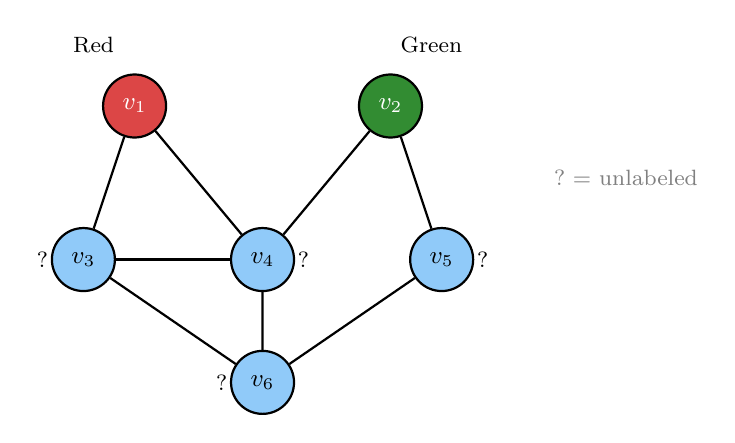
\begin{tikzpicture}[scale=1.3,
    labeled/.style={circle, draw, thick, minimum size=0.8cm, font=\small\bfseries,
      text=white},
    unlabeled/.style={circle, draw, thick, minimum size=0.8cm, font=\small,
      fill=unlabeledblue}]

    % Nodes
    \node[labeled, fill=labeledred] (1) at (0, 1.5) {$v_1$};
    \node[labeled, fill=labeledgreen] (2) at (2.5, 1.5) {$v_2$};
    \node[unlabeled] (3) at (-0.5, 0) {$v_3$};
    \node[unlabeled] (4) at (1.25, 0) {$v_4$};
    \node[unlabeled] (5) at (3, 0) {$v_5$};
    \node[unlabeled] (6) at (1.25, -1.2) {$v_6$};

    % Edges
    \draw[thick] (1) -- (3);
    \draw[thick] (1) -- (4);
    \draw[thick] (2) -- (4);
    \draw[thick] (2) -- (5);
    \draw[thick] (3) -- (4);
    \draw[thick] (3) -- (6);
    \draw[thick] (4) -- (6);
    \draw[thick] (5) -- (6);

    % Legend
    \node[draw=none, font=\footnotesize] at (-0.4, 2.1) {Red};
    \node[draw=none, font=\footnotesize] at (2.9, 2.1) {Green};
    \node[draw=none, font=\footnotesize] at (-0.9, 0) {?};
    \node[draw=none, font=\footnotesize] at (1.65, 0) {?};
    \node[draw=none, font=\footnotesize] at (3.4, 0) {?};
    \node[draw=none, font=\footnotesize] at (0.85, -1.2) {?};
    \node[draw=none, font=\footnotesize, text=gray] at (4.8, 0.8)
      {$?$ = unlabeled};
\end{tikzpicture}
\end{center}

\emph{Labelled set:} $\mathcal{V}_L = \{v_1, v_2\}$ (nodes come first after
reordering). \emph{Unlabelled set:} $\mathcal{V}_U = \{v_3, v_4, v_5, v_6\}$.

\emph{Label matrix} ($C = 2$ classes):
\[
Y = \begin{pmatrix} Y_L \\ \hline Y_U \end{pmatrix}
= \left(\begin{array}{cc} 1 & 0 \\ 0 & 1 \\ \hline 0 & 0 \\ 0 & 0 \\
0 & 0 \\ 0 & 0 \end{array}\right)
\quad \leftarrow \begin{array}{l} v_1 \text{ is Red} \\ v_2 \text{ is Green} \\
v_3 \text{ unknown} \\ v_4 \text{ unknown} \\ v_5 \text{ unknown} \\
v_6 \text{ unknown} \end{array}
\]

\emph{Adjacency matrix} (unweighted, so $A_{ij} \in \{0,1\}$), partitioned:
\[
A = \left(\begin{array}{cc|cccc}
0 & 0 & 1 & 1 & 0 & 0 \\
0 & 0 & 0 & 1 & 1 & 0 \\
\hline
1 & 0 & 0 & 1 & 0 & 1 \\
1 & 1 & 1 & 0 & 0 & 1 \\
0 & 1 & 0 & 0 & 0 & 1 \\
0 & 0 & 1 & 1 & 1 & 0
\end{array}\right)
= \begin{pmatrix} A_{LL} & A_{LU} \\ A_{UL} & A_{UU} \end{pmatrix}
\]

Reading the blocks: $A_{LU} = \bigl(\begin{smallmatrix} 1&1&0&0 \\ 0&1&1&0
\end{smallmatrix}\bigr)$ encodes which unlabelled nodes are neighbours of each
labelled node (e.g.\ $v_1$ connects to $v_3, v_4$). $A_{UU}$ encodes edges
among unlabelled nodes only.

\emph{Transition matrix} $P = D^{-1}A$ with $D = \diag(2, 2, 3, 4, 2, 3)$:
\[
P_{UL} = \begin{pmatrix} 1/3 & 0 \\ 1/4 & 1/4 \\ 0 & 1/2 \\ 0 & 0 \end{pmatrix},
\quad
P_{UU} = \begin{pmatrix} 0 & 1/3 & 0 & 1/3 \\ 1/4 & 0 & 0 & 1/4 \\
0 & 0 & 0 & 1/2 \\ 1/3 & 1/3 & 1/3 & 0 \end{pmatrix}
\]

\emph{Interpretation:} $P_{UL}$ tells us how much ``label information'' each
unlabelled node receives directly from labelled nodes. For instance, $v_4$ gets
$1/4$ of its weight from $v_1$ (Red) and $1/4$ from $v_2$ (Green). Node $v_6$
has $P_{v_6, L} = (0, 0)$: it receives \emph{no direct label information} ---
it can only be classified through multi-hop propagation via $P_{UU}$.
\end{example}


\section{Label propagation algorithms}
\label{semi-supervised-graphs:sec:lp}

We now turn to the central question of this chapter: given a graph with a
few labelled nodes and many unlabelled ones, how do we predict the labels of the
unlabelled nodes using only the graph structure (no node features)?

The core idea is remarkably intuitive: \emph{let each node adopt the
consensus of its neighbours}. If we repeat this averaging process --- while
keeping the labelled nodes fixed --- the label information gradually diffuses
through the graph until every node has a prediction. This is
\emph{label propagation}.

\begin{intuition}
\emph{Diffusion analogy.} Think of the graph as a network of pipes
connecting containers of water. Labelled nodes are faucets held at fixed
temperatures: class $A =$ ``hot'', class $B =$ ``cold''. At each time step,
every container equilibrates with its neighbours. Over time, the temperature
field reaches a smooth interpolation --- hot near class~$A$ sources, cold near
class~$B$, and tepid in between. Label propagation formalizes this process
using the transition matrix $P = D^{-1}A$ from
\cref{semi-supervised-graphs:subsec:random_walks}.
\end{intuition}

\subsection{Label propagation (Zhu and Ghahramani, 2002)}
\label{semi-supervised-graphs:subsec:lp_algo}

\begin{algorithm}[H]
\caption{Label propagation (Zhu and Ghahramani, 2002)}
\label{semi-supervised-graphs:alg:label_prop}
\begin{algorithmic}[1]
\State \textbf{Input:} Graph $G$, labelled set $\mathcal{V}_L$, labels $Y_L$,
        max iterations $T$, tolerance $\epsilon$
\State \textbf{Initialize:} $Y_U^{(0)} = \mathbf{0}$
\State Compute $P = D^{-1}A$
\For{$t = 1, 2, \ldots, T$}
    \State $Y^{(t)} = P \, Y^{(t-1)}$
      \Comment{Diffuse: each node averages its neighbours}
    \State $Y_L^{(t)} = Y_L$ \Comment{Clamp: reset labelled nodes}
    \If{$\|Y^{(t)} - Y^{(t-1)}\|_F < \epsilon$} \textbf{break} \EndIf
\EndFor
\State \textbf{Output:} $\hat{y}_i = \argmax_c Y_{ic}^{(T)}$ for
      $i \in \mathcal{V}_U$
\end{algorithmic}
\end{algorithm}

The algorithm alternates two operations. \emph{Diffuse} (step~5): every
node --- labelled and unlabelled --- replaces its current label distribution by the
weighted average of its neighbours' distributions. This is simply
multiplication by the transition matrix $P$. \emph{Clamp} (step~6): the
labelled nodes are reset to their known labels, undoing any change the
diffusion made to them.

Why is clamping necessary? Without it, the original labels would be diluted
and eventually lost --- every node would converge to the same global average.
Clamping ensures that labelled nodes act as permanent ``anchors'' that
continually inject label information into the graph.

In the block-partitioned form (\cref{semi-supervised-graphs:def:partitioning}), clamping
means the update for unlabelled nodes is:
\begin{equation}
\label{semi-supervised-graphs:eq:lp_update}
Y_U^{(t)} = P_{UL}\,Y_L + P_{UU}\,Y_U^{(t-1)}
\end{equation}
The first term $P_{UL}Y_L$ is the direct contribution from labelled neighbours
(constant across iterations, thanks to clamping). The second term
$P_{UU}Y_U^{(t-1)}$ is the contribution from other unlabelled neighbours,
which evolves over time.

\subsection{Convergence and closed-form solution}

Does the iteration~\eqref{semi-supervised-graphs:eq:lp_update} converge? If so, to what?

\begin{theorem}[Closed-form solution and convergence]
\label{semi-supervised-graphs:thm:lp_closed}
Let $G$ be a connected graph (\cref{semi-supervised-graphs:def:standing}) with at
least one labelled node. Then label propagation converges to
$Y_U^* = (I - P_{UU})^{-1}P_{UL}Y_L$.
\end{theorem}

\begin{pitfall}
\emph{Connectivity is essential.} This is the first place in the chapter
where connectivity is genuinely used. If $G$ is disconnected, consider an
unlabelled node $v_i$ in a connected component that contains \emph{no} labelled
nodes. Every neighbour of $v_i$ is also unlabelled, so
$\sum_{j \in \mathcal{V}_U}(P_{UU})_{ij} = \sum_j P_{ij} = 1$: no
probability leaks to labelled nodes. On such a component, $P_{UU}$ is
(fully) stochastic, $\rho(P_{UU}) = 1$, and the iteration does not converge.
In practice, if a graph has multiple connected components, label propagation
must be applied to each component separately, and any component without
labelled nodes cannot be classified by this method.
\end{pitfall}

\begin{proof}
We proceed in three steps, carefully ordering existence before convergence.
\vspace{0.5em}

\emph{Step 1: $\rho(P_{UU}) < 1$ and existence of $Y_U^*$.}
Since $P$ is row-stochastic ($\sum_j P_{ij} = 1$), the submatrix $P_{UU}$ has
row sums:
\[
\sum_{j \in \mathcal{V}_U} (P_{UU})_{ij}
= 1 - \underbrace{\sum_{j \in \mathcal{V}_L} P_{ij}}_{=:\,\ell_i} \;\leq\; 1,
\]
where $\ell_i \geq 0$ is the \emph{one-step escape probability} at $v_i$:
the probability that a random walker at $v_i$ jumps directly into
$\mathcal{V}_L$ in one step. Since $G$ is connected and has at least one
labelled node, every unlabelled node $v_i$ adjacent to a labelled node satisfies
$\ell_i > 0$, giving a strictly sub-unit row sum. A non-negative matrix whose
row sums are all $\leq 1$ with at least one strictly $< 1$ is called
\emph{sub-stochastic}. We show in \cref{semi-supervised-graphs:app:substochastic} that
sub-stochasticity together with connectivity implies $\rho(P_{UU}) < 1$.

Since $\rho(P_{UU}) < 1$, the matrix $I - P_{UU}$ is invertible
(all its eigenvalues $1 - \sigma_k$ satisfy $|1-\sigma_k| \geq 1 - \rho(P_{UU})
> 0$). We therefore \emph{define}:
\[
  Y_U^* \;:=\; (I - P_{UU})^{-1}\,P_{UL}\,Y_L.
\]

\emph{Step 2: $Y_U^*$ is a fixed point of the iteration.}
We verify by direct substitution that $Y_U^*$ satisfies the
update~\eqref{semi-supervised-graphs:eq:lp_update}:
\[
  P_{UL}Y_L + P_{UU}Y_U^*
  = P_{UL}Y_L + P_{UU}(I-P_{UU})^{-1}P_{UL}Y_L
  = \bigl(I + P_{UU}(I-P_{UU})^{-1}\bigr)P_{UL}Y_L.
\]
Using the identity $I + P_{UU}(I-P_{UU})^{-1} = (I-P_{UU})^{-1}$
(multiply both sides on the right by $(I-P_{UU})$ to verify), we get:
\[
  P_{UL}Y_L + P_{UU}Y_U^* = (I-P_{UU})^{-1}P_{UL}Y_L = Y_U^*.
\]
So $Y_U^*$ is indeed a fixed point. No circularity: we derived the fixed-point
equation from the explicit formula, not the other way around.

\emph{Step 3: the iteration converges to $Y_U^*$.}
Now that $Y_U^*$ exists and is verified to be a fixed point, define the error
$e^{(t)} := Y_U^{(t)} - Y_U^*$. Using~\eqref{semi-supervised-graphs:eq:lp_update} and the fixed-point
equation from Step~2:
\begin{align}
e^{(t)} &= Y_U^{(t)} - Y_U^* \notag\\
&= \bigl(P_{UL}Y_L + P_{UU}Y_U^{(t-1)}\bigr)
 - \bigl(P_{UL}Y_L + P_{UU}Y_U^*\bigr) \notag\\
&= P_{UU}\bigl(Y_U^{(t-1)} - Y_U^*\bigr) = P_{UU}\,e^{(t-1)}.
\end{align}
The $P_{UL}Y_L$ terms cancel because clamping keeps the labelled contribution
identical at every step. Applying the recurrence:
$e^{(t)} = P_{UU}^t\,e^{(0)}$.
Since $\rho(P_{UU}) < 1$, \cref{semi-supervised-graphs:prop:spectral_powers} gives
$P_{UU}^t \to 0$, hence $e^{(t)} \to 0$ and $Y_U^{(t)} \to Y_U^*$.
\end{proof}

\begin{remark}[Why use the iterative form in practice?]
\label{semi-supervised-graphs:rem:why_iterative}
The closed-form $Y_U^* = (I - P_{UU})^{-1}P_{UL}Y_L$ is elegant but
requires inverting a $u \times u$ matrix ($O(u^3)$ operations). For
$u = 10^6$ unlabelled nodes, this is intractable. By contrast, each iteration
of~\eqref{semi-supervised-graphs:eq:lp_update} costs only $O(|E| \cdot C)$ --- one sparse
matrix-vector product per class --- and convergence typically takes 10--50
iterations. The iterative form is therefore the practical choice for large
graphs.
\end{remark}

\subsection{The harmonic property}
\label{semi-supervised-graphs:subsec:harmonic}

The closed-form solution has an elegant mathematical characterization that
connects label propagation to a classical topic in mathematics:
\emph{harmonic functions} and \emph{boundary value problems}. This
perspective reveals that label propagation is not just a clever heuristic --- it
is the unique solution to a well-posed mathematical problem.

\subsubsection*{What does ``harmonic'' mean on a graph?}

In everyday language, a function is ``harmonic'' at a point if its value there
equals the average of its values nearby. On a graph, ``nearby'' means
``neighbours'':

\begin{definition}[Harmonic function on a graph]
\label{semi-supervised-graphs:def:harmonic}
A function $f: V \to \R$ is \emph{harmonic at node $v_i$} if its value
equals the weighted average of $f$ over the neighbours of $v_i$:
\begin{equation}
\label{semi-supervised-graphs:eq:harmonic_condition}
f(v_i) = \sum_{j \in \mathcal{N}(i)} \frac{A_{ij}}{d_i}\,f(v_j)
= \sum_j P_{ij}\,f(v_j)
\end{equation}
A function is \emph{harmonic on a set $S \subset V$} if it is harmonic at
every node in $S$.
\end{definition}

In other words, a harmonic function has \emph{no local extrema} on the
interior: no node can have a value strictly larger (or smaller) than all its
neighbours. Its value is always a compromise between its neighbours' values.
This is exactly what the diffusion process in label propagation produces --- the
iteration keeps averaging until every unlabelled node is at the ``consensus''
of its neighbourhood.

This is the graph version of the mean-value property of harmonic functions of \cref{ch:harmonic-functions}: equivalently, $(\mathcal L_{\mathrm{rw}}f)_i = f_i - \sum_jP_{ij}f_j = 0$, so harmonic at $v_i$ means in the kernel of the random-walk Laplacian at that node.

\subsubsection*{The boundary value problem}

In many physical problems, we know the value of a quantity on the boundary of
a region and want to find its values in the interior. For example: we know
the temperature on the walls of a room and want to find the steady-state
temperature at every point inside. This is a \emph{Dirichlet boundary value
problem}.

\begin{definition}[Dirichlet boundary value problem on a graph]
\label{semi-supervised-graphs:def:dirichlet}
Given a graph $G$, a set of \emph{boundary nodes} $\mathcal{V}_L$ with
prescribed values $f(v_i) = y_i$ for $i \in \mathcal{V}_L$, find a function
$f : V \to \R$ that is \emph{harmonic on the interior}
$\mathcal{V}_U = V \setminus \mathcal{V}_L$ while respecting the boundary
values.
\end{definition}

The parallel to semi-supervised learning is immediate: the boundary
nodes are the labelled nodes, the boundary values are the labels, and the
interior is the set of unlabelled nodes whose values we seek. Label
propagation is literally solving a boundary value problem on the graph.

\subsubsection*{Label propagation solves the Dirichlet problem}

\begin{proposition}[Harmonic property of label propagation]
\label{semi-supervised-graphs:prop:harmonic}
The label propagation solution $Y_U^*$ is harmonic on $\mathcal{V}_U$ with
Dirichlet boundary conditions $Y_L$. That is, label propagation solves the
discrete Dirichlet boundary value problem.
\end{proposition}

\begin{proof}
The proof is immediate from the fixed-point equation. At convergence, for
each unlabelled node $i \in \mathcal{V}_U$:
\[
Y_i^* = \sum_j P_{ij}\,Y_j^*
\]
This is precisely the harmonic condition
(\cref{semi-supervised-graphs:def:harmonic}). Meanwhile, the clamping step ensures
$Y_j^* = y_j$ for all $j \in \mathcal{V}_L$ (the Dirichlet boundary
condition).
\end{proof}

\subsubsection*{Worked example: verifying harmonicity}

To make this concrete, consider a small weighted triangle where we can check
every condition by hand.

\begin{figure}[ht]
\centering
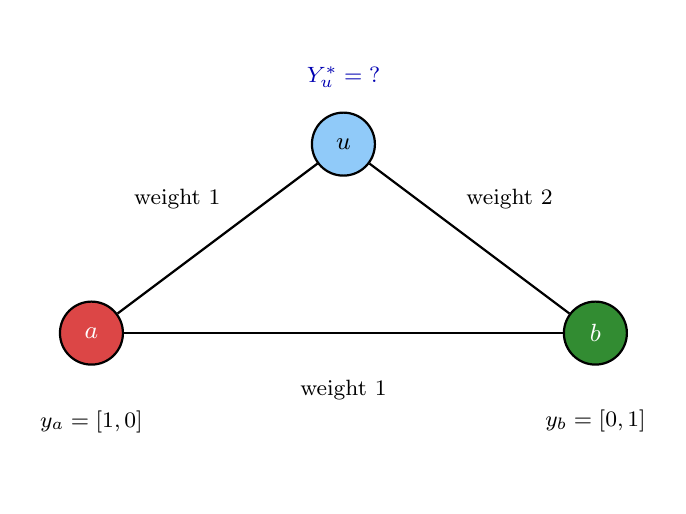
\begin{tikzpicture}[scale=1.6,
    every node/.style={circle, draw, minimum size=0.8cm, font=\small, thick}]
    \node[fill=labeledred, text=white, font=\small\bfseries] (A) at (0,0) {$a$};
    \node[fill=labeledgreen, text=white, font=\small\bfseries] (B) at (4,0) {$b$};
    \node[fill=unlabeledblue] (U) at (2,1.5) {$u$};

    \draw[thick] (A) -- node[below, draw=none, minimum size=0pt,
      font=\footnotesize] {weight 1} (B);
    \draw[thick] (A) -- node[above left, draw=none, minimum size=0pt,
      font=\footnotesize] {weight 1} (U);
    \draw[thick] (B) -- node[above right, draw=none, minimum size=0pt,
      font=\footnotesize] {weight 2} (U);

    \node[below=0.3cm, draw=none, font=\footnotesize] at (A)
      {$y_a = [1,0]$};
    \node[below=0.3cm, draw=none, font=\footnotesize] at (B)
      {$y_b = [0,1]$};
    \node[above=0.2cm, draw=none, font=\footnotesize, text=blue!70!black]
      at (U) {$Y_u^* = \;?$};
\end{tikzpicture}
\caption{Triangle graph with two labelled boundary nodes ($a$, $b$) and one
  unlabelled interior node ($u$). Edge weights are shown. The harmonic solution
  at $u$ must equal the weighted average of its neighbours' values.}
\label{semi-supervised-graphs:fig:harmonic_triangle}
\end{figure}

Node $u$ has degree $d_u = 1 + 2 = 3$ (sum of incident edge weights), so the
transition probabilities from $u$ are $P_{ua} = 1/3$ and $P_{ub} = 2/3$.
The harmonic condition (\cref{semi-supervised-graphs:def:harmonic}) requires:
\[
Y_u^* = P_{ua}\,y_a + P_{ub}\,y_b
= \tfrac{1}{3}\,[1,0] + \tfrac{2}{3}\,[0,1] = [\,1/3,\; 2/3\,]
\]
Node $u$ is predicted as class $B$ (Green) with probability $2/3$ --- reflecting
the fact that its edge to $b$ is twice as strong as its edge to $a$. The
stronger connection ``pulls'' $u$ towards $b$'s label, just as a heavier pipe
carries more heat from a heat source.

This is the unique harmonic function on $\{u\}$ with boundary values
$y_a = [1,0]$ and $y_b = [0,1]$. No other assignment to $u$ satisfies the
averaging property.

\begin{intuition}
\emph{Resistor network interpretation.} The connection between harmonic
functions and electrical circuits is classical. Each edge with weight $A_{ij}$
acts as a conductor with conductance $A_{ij}$ (resistance $1/A_{ij}$). The
labelled nodes are connected to batteries at fixed voltages (class
$A = 1\text{V}$, class $B = 0\text{V}$). By Kirchhoff's current law, the
current flowing into any interior node must equal the current flowing out;
this balance condition is precisely the harmonic
equation~\eqref{semi-supervised-graphs:eq:harmonic_condition}. Label propagation computes the
equilibrium voltages.

In the triangle above, node $u$ is connected to the $1$V source (node $a$)
by a conductor of conductance~$1$ and to the $0$V source (node $b$) by a
conductor of conductance~$2$. More current flows from $b$ (higher
conductance), pulling $u$'s voltage towards $0$V. The result,
$V_u = 1/3 \approx 0.33\text{V}$, is consistent with $Y_u^*[A] = 1/3$.
\end{intuition}

\subsection{Numerical example}
\label{semi-supervised-graphs:subsec:lp_example}

\begin{example}[Label propagation on a path graph]
\label{semi-supervised-graphs:ex:lp_path}
Consider the simplest interesting case: a path graph with five nodes, where
only the two endpoints are labelled.

\begin{center}
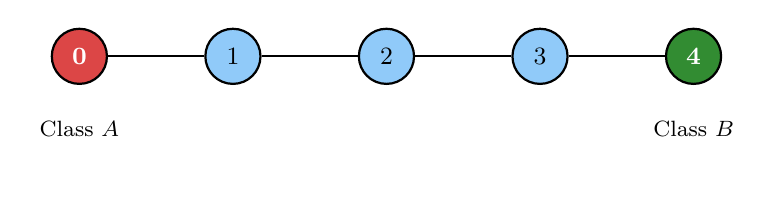
\begin{tikzpicture}[scale=1.5,
    every node/.style={circle, draw, minimum size=0.7cm, font=\small, thick}]
    \node[fill=labeledred, text=white, font=\small\bfseries] (0) at (0,0) {0};
    \node[fill=unlabeledblue] (1) at (1.3,0) {1};
    \node[fill=unlabeledblue] (2) at (2.6,0) {2};
    \node[fill=unlabeledblue] (3) at (3.9,0) {3};
    \node[fill=labeledgreen, text=white, font=\small\bfseries] (4) at (5.2,0) {4};
    \draw[thick] (0)--(1)--(2)--(3)--(4);
    \node[below=0.25cm, draw=none, font=\footnotesize] at (0) {Class $A$};
    \node[below=0.25cm, draw=none, font=\footnotesize] at (4) {Class $B$};
\end{tikzpicture}
\end{center}

The interior nodes $1, 2, 3$ are unlabelled. Since each interior node has
exactly two neighbours, the transition matrix gives equal weight $1/2$ to each:

$P_{UU} = \begin{psmallmatrix} 0 & 1/2 & 0 \\ 1/2 & 0 & 1/2 \\
0 & 1/2 & 0 \end{psmallmatrix}$, \;
$P_{UL} = \begin{psmallmatrix} 1/2 & 0 \\ 0 & 0 \\ 0 & 1/2 \end{psmallmatrix}$.

\noindent Note that $P_{UU}$ is sub-stochastic: the rows of nodes 1 and 3 sum
to $1/2$ (they each have a labelled neighbour), while node~2's row sums to~1
(both neighbours are unlabelled). Nonetheless, since node~2 can reach a labelled
node in two steps, the walk eventually escapes, and $\rho(P_{UU}) < 1$.

Solving $(I - P_{UU})Y_U^* = P_{UL}I_2$:

\[
(I - P_{UU})^{-1} = \begin{pmatrix}
3/2 & 1 & 1/2 \\ 1 & 2 & 1 \\ 1/2 & 1 & 3/2
\end{pmatrix} \implies
Y_U^* = \begin{pmatrix} 3/4 & 1/4 \\ 1/2 & 1/2 \\ 1/4 & 3/4 \end{pmatrix}
\]

\begin{center}
\begin{tabular}{c|cc|c}
\toprule Node & $P(A)$ & $P(B)$ & Prediction \\ \midrule
0 & 1.00 & 0.00 & $A$ (given) \\
1 & 0.75 & 0.25 & $A$ \\
2 & 0.50 & 0.50 & Tie \\
3 & 0.25 & 0.75 & $B$ \\
4 & 0.00 & 1.00 & $B$ (given) \\ \bottomrule
\end{tabular}
\end{center}

The result is a linear interpolation between the two boundary labels --- exactly
what the diffusion analogy predicts. We can verify the harmonic property at
node~2: $Y_2^* = \frac{1}{2}Y_1^* + \frac{1}{2}Y_3^*
= \frac{1}{2}(3/4,1/4) + \frac{1}{2}(1/4,3/4) = (1/2,1/2)$.

The random walk interpretation (\cref{semi-supervised-graphs:subsec:random_walks}) also
applies: a walk starting at node~1 reaches node~0 (class $A$) before node~4
(class $B$) with probability $3/4$.
\end{example}

\subsection{Label spreading (Zhou et al., 2004)}
\label{semi-supervised-graphs:subsec:ls}

Label propagation's hard clamping means that if a labelled node has an
\emph{incorrect} label (noise), this error propagates permanently through the
graph. Label spreading (Zhou et al., \emph{Learning with Local and Global Consistency}, 2004) introduces \emph{soft clamping}:
labelled nodes can be updated by the diffusion, but a ``spring'' force pulls
them back towards their initial values:

\begin{algorithm}[H]
\caption{Label spreading (Zhou et al., 2004)}
\begin{algorithmic}[1]
\State \textbf{Input:} Graph $G$, initial labels $Y^{(0)}$, parameter
      $\alpha \in (0,1)$, tolerance $\epsilon$
\State Compute $S = D^{-1/2}AD^{-1/2}$
\For{$t = 1, 2, \ldots$}
    \State $Y^{(t)} = \alpha\, S\, Y^{(t-1)} + (1-\alpha)\, Y^{(0)}$
    \If{$\|Y^{(t)} - Y^{(t-1)}\|_F < \epsilon$} \textbf{break} \EndIf
\EndFor
\State \textbf{Output:} $\hat{y}_i = \argmax_c Y_{ic}^{(T)}$
\end{algorithmic}
\end{algorithm}

\paragraph{Key differences from label propagation.}
\begin{itemize}
    \item Uses $S = D^{-1/2}AD^{-1/2}$ (symmetric, degree-normalized)
    instead of $P = D^{-1}A$ (row-stochastic).
    \item Even labelled nodes are updated; the term $(1{-}\alpha)Y^{(0)}$
    pulls them back towards initial values. Parameter $\alpha \to 1$:
    trust graph more; $\alpha \to 0$: trust labels more.
\end{itemize}

\begin{theorem}[Label spreading: closed form and convergence]
\label{semi-supervised-graphs:thm:ls_closed}
Label spreading converges to $Y^* = (1-\alpha)(I - \alpha S)^{-1}Y^{(0)}$, and
the inverse exists for all $\alpha \in (0,1)$.
\end{theorem}

\begin{proof}
We follow the same logical order as in \cref{semi-supervised-graphs:thm:lp_closed}: first
establish existence of $Y^*$ by direct construction, then verify it is a fixed
point, then prove the iteration converges to it.
\vspace{0.5em}

\emph{Step 1: invertibility of $I - \alpha S$ and existence of $Y^*$.}
By \cref{semi-supervised-graphs:prop:normalized_properties}(3), the eigenvalues $\sigma_k$
of $S$ satisfy $\sigma_k \in [-1, 1]$. Hence the eigenvalues of $\alpha S$ lie
in $[-\alpha, \alpha]$, and those of $I - \alpha S$ lie in
$[1-\alpha,\, 1+\alpha] \subset (0, 2)$ for any $\alpha \in (0,1)$. Since all
eigenvalues are strictly positive, $I - \alpha S$ is positive definite, hence
invertible. We therefore \emph{define}:
\[
  Y^* \;:=\; (1-\alpha)(I - \alpha S)^{-1}\,Y^{(0)}.
\]

\emph{Step 2: $Y^*$ is a fixed point of the iteration.}
We verify by direct substitution that $Y^*$ satisfies the update
$Y = \alpha S Y + (1-\alpha)Y^{(0)}$:
\[
  \alpha S Y^* + (1-\alpha)Y^{(0)}
  = \alpha S\,(1-\alpha)(I-\alpha S)^{-1}Y^{(0)} + (1-\alpha)Y^{(0)}
  = (1-\alpha)\bigl(\alpha S(I-\alpha S)^{-1} + I\bigr)Y^{(0)}.
\]
Using the identity $I + \alpha S(I - \alpha S)^{-1} = (I - \alpha S)^{-1}$
(multiply both sides on the right by $(I - \alpha S)$ to verify), we get:
\[
  \alpha S Y^* + (1-\alpha)Y^{(0)}
  = (1-\alpha)(I - \alpha S)^{-1}Y^{(0)} = Y^*.
\]
So $Y^*$ is indeed a fixed point, derived from its explicit formula without
any circularity.

\emph{Step 3: the iteration converges to $Y^*$.}
Now that $Y^*$ exists and is a fixed point, define $e^{(t)} := Y^{(t)} - Y^*$.
Using the update rule and the fixed-point equation from Step~2:
\begin{align}
e^{(t)} &= Y^{(t)} - Y^* \notag\\
&= \bigl(\alpha S Y^{(t-1)} + (1-\alpha)Y^{(0)}\bigr)
 - \bigl(\alpha S Y^* + (1-\alpha)Y^{(0)}\bigr) \notag\\
&= \alpha S\bigl(Y^{(t-1)} - Y^*\bigr) = \alpha S\,e^{(t-1)}.
\end{align}
The $(1-\alpha)Y^{(0)}$ terms cancel identically at every step. Applying the
recurrence: $e^{(t)} = (\alpha S)^t\,e^{(0)}$. Since $\rho(\alpha S) \leq
\alpha < 1$, \cref{semi-supervised-graphs:prop:spectral_powers} gives $(\alpha S)^t \to 0$,
hence $e^{(t)} \to 0$ and $Y^{(t)} \to Y^*$.
\end{proof}

\begin{theorem}[Variational formulation]
\label{semi-supervised-graphs:thm:ls_energy}
Label spreading minimizes a well-defined energy function that balances two
competing objectives:
\begin{equation}
\mathcal{E}(F) =
\underbrace{\sum_{\{i,j\}\in E} A_{ij}\left(\frac{F_i}{\sqrt{d_i}} -
\frac{F_j}{\sqrt{d_j}}\right)^2}_{\mathclap{\substack{
    \text{normalized smoothness:}\\
    \text{``nearby nodes should agree''}}}} \; + \; \frac{1-\alpha}{\alpha}\,
\underbrace{\sum_{i=1}^n \|F_i - Y_i^{(0)}\|^2}_{\mathclap{\substack{
    \text{label fitting:}\\
    \text{``do not stray from initial labels''}}}}
\end{equation}
\end{theorem}

This variational perspective is important for two reasons. First, it shows
that label spreading is not merely an ad hoc iterative scheme --- it is solving
a principled optimization problem with a clear objective. Second, the two
terms reveal the trade-off controlled by $\alpha$: when $\alpha$ is large, the
smoothness term dominates and the solution follows the graph structure; when
$\alpha$ is small, the fitting term dominates and the solution stays close to
the initial labels.

\begin{proof}
See \cref{semi-supervised-graphs:app:ls_energy}.
\end{proof}

\section{Correct and smooth}
\label{semi-supervised-graphs:sec:cs}

Label propagation and label spreading operate directly on the label matrix
$Y$. But what if we already have a powerful base predictor (e.g.\ a neural
network trained on node features) that produces soft predictions
$\hat{Y} \in \R^{n \times C}$? Can we use the graph to \emph{correct} and
\emph{smooth} these predictions without retraining?

Correct and Smooth (C\&S) (Huang et al., \emph{Combining Label Propagation and Simple Models Out-performs Graph Neural Networks}, 2021) answers this question with a
surprisingly simple and effective two-stage post-processing method. It has
become a standard component in many graph learning pipelines, often providing
substantial improvements at near-zero additional cost.

\begin{intuition}
\emph{Core idea:} Base model predictions contain systematic errors that are
\emph{correlated along graph edges}. If node $v$ misclassifies, its neighbours
likely make similar mistakes. We can estimate these errors from labelled nodes
and propagate them to correct unlabelled nodes. Then we smooth the corrected
predictions to enforce local consistency.
\end{intuition}

\subsection{Intuition: errors are contagious}

Consider a simple binary classification problem on a graph with high homophily.
A base model (e.g.\ a multilayer perceptron trained only on node features)
produces predictions $\hat{y}_i \in [0,1]$ for each node. On labelled nodes, we
can compute the \emph{training error}:
\begin{equation}
E_i = y_i - \hat{y}_i \quad \text{for } i \in \mathcal{V}_L
\end{equation}

These errors are not random noise --- they reflect systematic biases in the base
model. Crucially, due to homophily, if the base model under-predicts the
probability of class $A$ for a labelled node, it likely under-predicts for that
node's neighbours as well. Therefore, we can \emph{propagate} these errors
from labelled to unlabelled nodes to correct their predictions.

\subsection{Stage 1: correcting predictions}

Let $\hat{Y} \in \R^{n \times C}$ be the base model's soft predictions
(typically logits or probabilities). Define the \emph{error matrix}
$E \in \R^{n \times C}$ where:
\begin{equation}
E_{i} = \begin{cases}
Y_i - \hat{Y}_i & \text{if } i \in \mathcal{V}_L \\
\mathbf{0} & \text{if } i \in \mathcal{V}_U
\end{cases}
\end{equation}

We now propagate these errors using $k$ steps of label propagation with the
normalized adjacency $S = D^{-1/2}AD^{-1/2}$:

\begin{keyidea}
\emph{Error propagation:}
\begin{equation}
E^{(0)} = E, \quad E^{(t+1)} = (1-\alpha) E + \alpha S E^{(t)}
\end{equation}
or equivalently in closed form:
\begin{equation}
E^* = (1-\alpha)(I - \alpha S)^{-1} E
\end{equation}

The corrected predictions are:
\begin{equation}
\hat{Y}^{\text{corr}} = \hat{Y} + E^*
\end{equation}
\end{keyidea}

The hyperparameter $\alpha \in (0,1)$ controls how much error information flows
from labelled nodes. Higher $\alpha$ means longer-range propagation. In practice,
$k$ is often set to a small integer (e.g.\ 5--10) rather than iterating to
convergence.

\begin{remark}[Why propagate errors, not labels?]
Directly propagating labels (as in label propagation) ignores the base model's
predictions entirely. C\&S preserves the base model's output and only corrects
its \emph{residuals}. This is analogous to boosting: we fit a model to the
errors of a base learner.
\end{remark}

\subsection{Stage 2: smoothing predictions}

After correction, the predictions $\hat{Y}^{\text{corr}}$ may still be noisy
and not locally consistent. The smoothing stage applies another round of
diffusion, this time on the corrected predictions themselves:

\begin{keyidea}
\emph{Prediction smoothing:}
\begin{equation}
Z^{(0)} = \hat{Y}^{\text{corr}}, \quad Z^{(t+1)} = (1-\beta) \hat{Y}^{\text{corr}} + \beta S Z^{(t)}
\end{equation}
or in closed form:
\begin{equation}
Z^* = (1-\beta)(I - \beta S)^{-1} \hat{Y}^{\text{corr}}
\end{equation}
\end{keyidea}

Why smooth after correcting? The correction step adds a propagated error signal
that may be noisy, especially for nodes far from labelled examples. Smoothing
enforces that neighbouring nodes have similar predictions, leveraging the graph
homophily assumption.

\begin{pitfall}
\emph{Critical:} Smoothing uses $\hat{Y}^{\text{corr}}$ as the ``base''
predictions, not $\hat{Y}$. The term $(1-\beta)\hat{Y}^{\text{corr}}$ in each
iteration pulls the smoothed predictions back towards the \emph{corrected} values,
not the original noisy predictions. This prevents the smoothing step from
undoing the correction.
\end{pitfall}

\subsection{Mathematical justification}

C\&S can be understood as solving two separate graph-regularized optimization
problems, each of the same form as label spreading
(\cref{semi-supervised-graphs:thm:ls_energy}). This variational perspective reveals \emph{why}
the two-stage pipeline is principled: both stages are not ad hoc diffusion
steps, but optimal solutions to well-posed smoothness problems.

\subsubsection*{The common structure}

Both stages minimize an objective of the form
\begin{equation}
\label{semi-supervised-graphs:eq:cs_general_opt}
\min_{F \in \R^{n \times C}}\;
\underbrace{\|F - B\|_F^2}_{\text{stay close to }B}
\;+\; \mu \underbrace{\sum_{\{i,j\}\in E}A_{ij}
\left\|\frac{F_i}{\sqrt{d_i}} - \frac{F_j}{\sqrt{d_j}}\right\|^2}_{
\mathclap{=\,\tr(F^\top \mathcal{L}_{\mathrm{sym}} F)}}
\end{equation}
for a ``target'' matrix $B$ and a trade-off parameter $\mu > 0$, the sum running over edges (each counted once). Its unique minimizer is $(I + \mu\,\mathcal{L}_{\mathrm{sym}})^{-1}B$, which equals the label-spreading form $(1-\alpha)(I - \alpha S)^{-1}B$ for $\alpha = \mu/(1+\mu)$, that is $\mu = \alpha/(1-\alpha)$ (proof in \cref{semi-supervised-graphs:app:cs_opt}). The two stages of C\&S are instances of this template with different targets $B$.

\begin{theorem}[Correct step as optimization]
\label{semi-supervised-graphs:thm:cs_correct_opt}
The error propagation $E^* = (1-\alpha)(I - \alpha S)^{-1}E$ is the unique
minimizer of:
\begin{equation}
\min_{F \in \R^{n \times C}}\; \|F - E\|_F^2
  + \frac{\alpha}{1-\alpha}\sum_{\{i,j\}\in E}A_{ij}
  \left\|\frac{F_i}{\sqrt{d_i}} - \frac{F_j}{\sqrt{d_j}}\right\|^2
\end{equation}
That is, $E^*$ is the smoothest signal (in the normalized-Laplacian sense) that
remains close to the observed error matrix $E$. Since $E$ is non-zero only on
labelled nodes, the optimization spreads these errors to unlabelled nodes via the
graph structure.
\end{theorem}

\begin{theorem}[Smooth step as optimization]
\label{semi-supervised-graphs:thm:cs_smooth_opt}
The smoothed predictions $Z^* = (1-\beta)(I - \beta S)^{-1}\hat{Y}^{\text{corr}}$
are the unique minimizer of:
\begin{equation}
\min_{F \in \R^{n \times C}}\; \|F - \hat{Y}^{\text{corr}}\|_F^2
  + \frac{\beta}{1-\beta}\sum_{\{i,j\}\in E}A_{ij}
  \left\|\frac{F_i}{\sqrt{d_i}} - \frac{F_j}{\sqrt{d_j}}\right\|^2
\end{equation}
That is, $Z^*$ is the smoothest signal that stays close to the corrected
predictions $\hat{Y}^{\text{corr}}$.
\end{theorem}

Both theorems are proved in \cref{semi-supervised-graphs:app:cs_opt}. The proofs follow the
same template as the label spreading energy proof
(\cref{semi-supervised-graphs:app:ls_energy}): compute the gradient, show it vanishes at the
claimed solution, and verify the Hessian is positive definite.

\begin{intuition}
\emph{What the variational view adds.} Beyond formal justification, the
variational formulation clarifies the role of $\alpha$ and $\beta$: they are
not arbitrary damping parameters but control the trade-off between fidelity to
the input ($\|F - B\|_F^2$) and graph smoothness. A large $\alpha$ (close to
1) makes the smoothness term cheap relative to fidelity, allowing the error
signal to spread far across the graph; a small $\alpha$ confines corrections to
nodes near labelled examples. The two stages are therefore interpretable as
independent regularized least-squares problems with a shared graph prior.
\end{intuition}

\subsection{Numerical example}
\begin{figure}[ht]
\centering
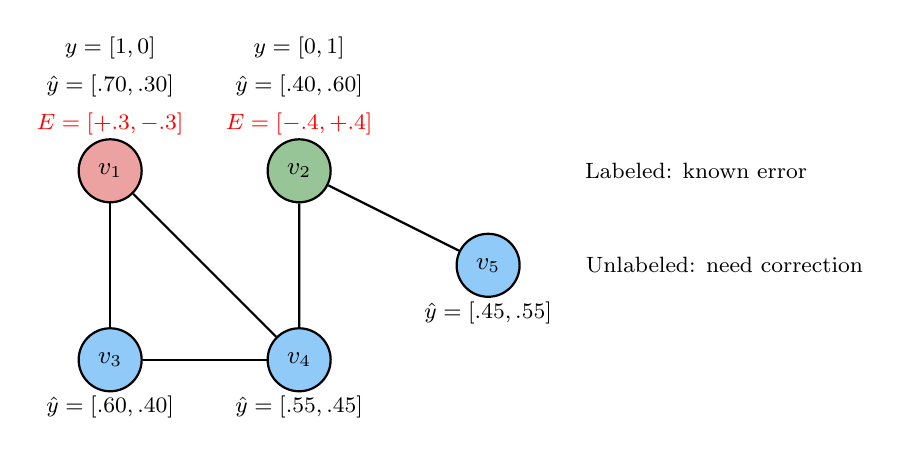
\begin{tikzpicture}[scale=1.2,
    node/.style={circle, draw, thick, minimum size=0.8cm, font=\small}]

    % Graph structure
    \node[node, fill=labeledred!50] (1) at (0,2) {$v_1$};
    \node[node, fill=labeledgreen!50] (2) at (2,2) {$v_2$};
    \node[node, fill=unlabeledblue] (3) at (0,0) {$v_3$};
    \node[node, fill=unlabeledblue] (4) at (2,0) {$v_4$};
    \node[node, fill=unlabeledblue] (5) at (4,1) {$v_5$};

    \draw[thick] (1) -- (3);
    \draw[thick] (1) -- (4);
    \draw[thick] (2) -- (4);
    \draw[thick] (2) -- (5);
    \draw[thick] (3) -- (4);

    % Labels and predictions
    \node[draw=none, font=\footnotesize] at (0,3.3) {$y=[1,0]$};
    \node[draw=none, font=\footnotesize] at (0,2.9) {$\hat{y}=[.70,.30]$};
    \node[draw=none, font=\footnotesize] at (2,3.3) {$y=[0,1]$};
    \node[draw=none, font=\footnotesize] at (2,2.9) {$\hat{y}=[.40,.60]$};
    \node[draw=none, font=\footnotesize] at (0,-0.5) {$\hat{y}=[.60,.40]$};
    \node[draw=none, font=\footnotesize] at (2,-0.5) {$\hat{y}=[.55,.45]$};
    \node[draw=none, font=\footnotesize] at (4,0.5) {$\hat{y}=[.45,.55]$};

    % Errors
    \node[draw=none, font=\footnotesize, text=red] at (0,2.5) {$E=[+.3,-.3]$};
    \node[draw=none, font=\footnotesize, text=red] at (2,2.5) {$E=[-.4,+.4]$};

    % Legend
    \node[draw=none, font=\footnotesize] at (6.2,2) {Labeled: known error};
    \node[draw=none, font=\footnotesize] at (6.5,1) {Unlabeled: need correction};
\end{tikzpicture}
\caption{C\&S setup. Degrees: $d_1 = d_2 = d_3 = 2$, $d_4 = 3$, $d_5 = 1$.}
\label{semi-supervised-graphs:fig:cs_error}
\end{figure}

Consider the 5-node graph from \cref{semi-supervised-graphs:fig:cs_error}. A base model
trained on node features produces predictions $\hat{Y}$ (shown). We apply
C\&S with $\alpha = \beta = 0.7$.
\vspace{0.5em}

\paragraph{Step 1: correct.} The error matrix $E$ is non-zero only on labelled
nodes: $E_1 = [+0.3, -0.3]$ (base model under-predicts Red for $v_1$),
$E_2 = [-0.4, +0.4]$ (under-predicts Green for $v_2$). Error propagation
via $E^{(t+1)} = 0.3\,E + 0.7\,S\,E^{(t)}$ spreads these errors through
the graph. To understand how, consider the first iteration. The product
$S\,E$ gives the error that each unlabelled node receives from its neighbours:
\begin{itemize}
    \item $v_3$ (neighbours: $v_1, v_4$) receives $[+0.15, -0.15]$ --- mainly
          from $v_1$'s positive Red error. Since $v_4$ has no error yet,
          only $v_1$ contributes.
    \item $v_4$ (neighbours: $v_1, v_2, v_3$) receives $[{-0.04}, {+0.04}]$.
          This small value arises because $v_1$'s error
          $S_{41}\!\cdot\![+0.3,-0.3] = [+0.12, -0.12]$ and $v_2$'s error
          $S_{42}\!\cdot\![-0.4,+0.4] = [-0.16, +0.16]$ \emph{partially
          cancel}. Node $v_4$ sits between the two labelled nodes, so the
          opposing corrections nearly neutralize.
    \item $v_5$ (neighbour: $v_2$ only) receives $[-0.28, +0.28]$ --- a strong
          correction towards Green, because $v_5$ is connected only to $v_2$.
\end{itemize}
After convergence, the propagated errors $E^*$ are added to $\hat{Y}$
and labelled nodes are clamped to their true labels.
\vspace{0.5em}

\paragraph{Step 2: smooth.} Smoothing via
$Z^{(t+1)} = 0.3\,\hat{Y}^{\text{corr}} + 0.7\,S\,Z^{(t)}$ averages
each node's prediction with its neighbours' corrected predictions:
\begin{itemize}
    \item $v_1$ (neighbours: $v_3, v_4$): pulled from $[1.00, 0.00]$
          (clamped) towards the average of $v_3$ and $v_4$'s corrected
          predictions $([0.63 + 0.54]/2 \approx 0.59$), yielding
          $[0.72, 0.28]$. Still Red, but the extreme clamped value is
          softened.
    \item $v_2$ (neighbours: $v_4, v_5$): pulled from $[0.00, 1.00]$
          (clamped) towards $v_4$ and $v_5$'s corrected values, yielding
          $[0.30, 0.70]$.
    \item $v_3$ (neighbours: $v_1, v_4$): its corrected prediction
          $[0.63, 0.37]$ already agrees well with its neighbours
          ($v_1$~is~Red, $v_4$~is~mixed), so smoothing barely changes it:
          $[0.63, 0.37]$.
    \item $v_4$ (neighbours: $v_1, v_2, v_3$): neighbour average is
          $[0.54, 0.46]$, close to $v_4$'s corrected prediction. Smoothing
          leaves it at $[0.54, 0.46]$ --- balanced between the two classes,
          reflecting its position between the two labelled nodes.
    \item $v_5$ (neighbour: $v_2$ only): pulled further towards Green,
          from $[0.37, 0.63] \to [0.33, 0.67]$. Smoothing reinforces the
          correction.
\end{itemize}

The complete pipeline is summarized in the following table. Because $S$ is not stochastic (\cref{semi-supervised-graphs:rem:row_sums}), the smoothed scores $Z^*$ do not sum to $1$ per row; for instance $Z^*_4 = (0.622, 0.523)$. The last column shows them renormalized row by row, which does not change the predicted classes. The numbers are computed by the script of \cref{semi-supervised-graphs:app:code}.

\begin{center}
\small
\resizebox{\linewidth}{!}{%
\begin{tabular}{c|c|c|c|c|c|c}
\toprule
Node & True & Base $\hat{Y}$ & Error $E$ & $E^*$ (propagated)
  & Corrected $\hat{Y}^{\text{corr}}$ & Smoothed $Z^*$ (normalized) \\
\midrule
$v_1$ (R) & [1,0] & [.70,\,.30] & [+.30,$-$.30] & ---
  & [1.00,\,0.00] (clamp) & [\textbf{.72},\,.28] \\
$v_2$ (G) & [0,1] & [.40,\,.60] & [$-$.40,+.40] & ---
  & [0.00,\,1.00] (clamp) & [.30,\,\textbf{.70}] \\
$v_3$ & ? & [.60,\,.40] & [0,\,0] & [+.03,$-$.03]
  & [\textbf{.63},\,.37] & [\textbf{.63},\,.37] \\
$v_4$ & ? & [.55,\,.45] & [0,\,0] & [$-$.01,+.01]
  & [.54,\,.46] & [.54,\,.46] \\
$v_5$ & ? & [.45,\,.55] & [0,\,0] & [$-$.08,+.08]
  & [.37,\,\textbf{.63}] & [.33,\,\textbf{.67}] \\
\bottomrule
\end{tabular}%
}
\end{center}
(Smoothed values are row-normalized. Bold marks the predicted class.)

The key observations: $v_5$'s initial weak lean towards Green ($[0.45, 0.55]$)
has been strengthened to a confident $[0.33, 0.67]$ through both correction and
smoothing. Node $v_4$, sitting between the two labelled nodes, receives almost
no net correction ($E^* \approx 0$) because the opposing errors cancel --- and
smoothing confirms this balanced position. Node $v_3$, connected to $v_1$ (Red)
but not $v_2$, is pulled towards Red by both stages.

\subsection{Why C\&S works so well}

C\&S achieves state-of-the-art results on many benchmarks with a simple linear
base model. Why?

\begin{enumerate}
    \item \textbf{Decouples feature learning from graph exploitation.}
          The base model learns from features without being distracted by graph
          structure; C\&S then optimally uses the graph to clean up predictions.
    \item \textbf{Avoids over-smoothing.} Unlike GCNs which mix features and
          graph in every layer, C\&S applies only two shallow diffusion steps,
          preventing the node representations from becoming indistinguishable.
    \item \textbf{Computational efficiency.} C\&S requires only sparse matrix
          multiplications and no gradient computation. It scales to graphs with
          billions of edges.
    \item \textbf{Principled diffusions.} Both stages are label-spreading problems with explicit objectives (\cref{semi-supervised-graphs:eq:cs_general_opt}), so their behaviour is controlled by two interpretable parameters. Huang et al.\ (\emph{Combining Label Propagation and Simple Models Out-performs Graph Neural Networks}, 2021) report that an MLP or linear model followed by C\&S matches or beats GNNs on several large benchmarks with far fewer parameters.
\end{enumerate}

\begin{intuition}
\emph{Takeaway:} Before training a complex GNN, try this recipe:
\begin{enumerate}
    \item Train a simple MLP on node features (ignore the graph).
    \item Apply C\&S to the MLP's predictions.
\end{enumerate}
This simple pipeline often outperforms sophisticated GNNs, especially when
features are informative and the graph is moderately homophilic.
\end{intuition}


\section{Graph regularization methods}
\label{semi-supervised-graphs:sec:reg}

The label propagation methods of \cref{semi-supervised-graphs:sec:lp} and the post-processing
of \cref{semi-supervised-graphs:sec:cs} use \emph{only} the graph structure to classify nodes
or correct predictions --- they either ignore node features entirely or treat
them only through a base model. In many applications (text classification,
molecular property prediction), rich features $x_i \in \R^d$ are available at
each node. How can we combine features with graph structure in a single
end-to-end training objective?

The idea is natural: train a parametric model $f_\theta$ (neural network, SVM,
etc.) on the labelled data as usual, but add a penalty term that discourages
$f_\theta$ from assigning different predictions to connected nodes. This
penalty is the Laplacian quadratic form from \cref{semi-supervised-graphs:thm:laplacian_quadratic},
which we already know measures how much a signal varies across edges.

\subsection{General framework}

\begin{definition}[Graph-regularized objective]
\label{semi-supervised-graphs:def:graph_reg}
For a parametric model $f_\theta: \R^d \to \R^C$ mapping node features to
class scores:
\begin{equation}
\label{semi-supervised-graphs:eq:graph_reg}
\mathcal{L}(\theta) =
\underbrace{
    \sum_{i \in \mathcal{V}_L}\ell(f_\theta(x_i), y_i)}_{
        \mathclap{\substack{\text{supervised loss} \\
        \text{(labelled nodes only)}}}} \; + \;
\lambda\underbrace{\frac{1}{2}\sum_{i,j}A_{ij}\|f_\theta(x_i) -
f_\theta(x_j)\|^2}_{\mathclap{\substack{\text{graph smoothness} \\
\text{(all nodes, labelled and unlabelled)}}}}
\end{equation}
where $\lambda > 0$ controls the regularization strength.
\end{definition}

The first term is standard supervised learning. The second term involves
\emph{all} nodes (labelled and unlabelled) --- this is how unlabelled data enters
the training. Minimizing it pushes the model towards predictions that are smooth
over the graph. We now make precise the connection to the Laplacian.

\begin{remark}[Graph regularizer as a trace form]
\label{semi-supervised-graphs:rem:trace_form}
Define $F \in \R^{n \times C}$ as the matrix whose $i$-th row is
$f_\theta(x_i)^\top \in \R^C$. The graph smoothness term in~\eqref{semi-supervised-graphs:eq:graph_reg}
can be written compactly as:
\begin{equation}
\label{semi-supervised-graphs:eq:trace_form}
\frac{1}{2}\sum_{i=1}^n\sum_{j=1}^n A_{ij}\|f_\theta(x_i) - f_\theta(x_j)\|^2
= \tr(F^\top L F).
\end{equation}
\emph{Derivation.} Expanding the squared norm class-by-class:
\[
\frac{1}{2}\sum_{i,j}A_{ij}\|F_i - F_j\|^2
= \frac{1}{2}\sum_{i,j}A_{ij}\sum_{c=1}^C(F_{ic}-F_{jc})^2
= \sum_{c=1}^C \frac{1}{2}\sum_{i,j}A_{ij}(F_{ic}-F_{jc})^2.
\]
By \cref{semi-supervised-graphs:thm:laplacian_quadratic}, each inner sum equals $f_c^\top L f_c$
where $f_c \in \R^n$ is the $c$-th column of $F$. Summing over $c$:
\[
\sum_{c=1}^C f_c^\top L f_c = \tr(F^\top L F),
\]
since $\tr(F^\top L F) = \sum_c (F^\top L F)_{cc} = \sum_c f_c^\top L f_c$. The
identity~\eqref{semi-supervised-graphs:eq:trace_form} thus follows directly from the scalar quadratic
form of \cref{semi-supervised-graphs:thm:laplacian_quadratic}, applied column by column.
\end{remark}

\begin{example}[Symbolic computation of $\tr(F^\top LF)$]
\label{semi-supervised-graphs:ex:trace_form_symbolic}
To make \cref{semi-supervised-graphs:rem:trace_form} concrete, consider a 3-node path graph
$v_1 - v_2 - v_3$ with unit edge weights ($A_{12} = A_{23} = 1$, all others
zero) and a model with $C = 2$ output classes. The degree matrix and Laplacian
are:
\[
D = \begin{pmatrix} 1 & 0 & 0 \\ 0 & 2 & 0 \\ 0 & 0 & 1 \end{pmatrix}, \qquad
L = D - A = \begin{pmatrix} 1 & -1 & 0 \\ -1 & 2 & -1 \\ 0 & -1 & 1 \end{pmatrix}.
\]
Let the model's output matrix $F \in \R^{3 \times 2}$ be written in terms of
symbolic scores:
\[
F = \begin{pmatrix} a_1 & b_1 \\ a_2 & b_2 \\ a_3 & b_3 \end{pmatrix},
\]
where $F_i = (a_i, b_i)^\top$ is the score vector output by $f_\theta$ at node
$v_i$ (e.g.\ the pre-softmax logits for classes $A$ and $B$).

\emph{Edge-sum formula.} The two edges of the graph contribute:
\begin{align*}
\frac{1}{2}\sum_{i,j}A_{ij}\|F_i - F_j\|^2
&= A_{12}\|F_1 - F_2\|^2 + A_{23}\|F_2 - F_3\|^2 \\
&= (a_1 - a_2)^2 + (b_1 - b_2)^2
 + (a_2 - a_3)^2 + (b_2 - b_3)^2.
\end{align*}
(Each unordered edge $\{i,j\}$ appears once because the $\frac{1}{2}$ cancels
the double-counting from the double sum, as in \cref{semi-supervised-graphs:thm:laplacian_quadratic}.)

\emph{Trace formula.} We verify that $\tr(F^\top LF)$ gives the same result.
Denote the two columns of $F$ as $f_A = (a_1, a_2, a_3)^\top$ and
$f_B = (b_1, b_2, b_3)^\top$. Then:
\begin{align*}
\tr(F^\top LF) &= f_A^\top L f_A + f_B^\top L f_B.
\end{align*}
Computing $f_A^\top L f_A$ using $L = D - A$:
\begin{align*}
f_A^\top L f_A
&= a_1^2 + 2a_2^2 + a_3^2 - 2a_1 a_2 - 2a_2 a_3 \\
&= (a_1 - a_2)^2 + (a_2 - a_3)^2,
\end{align*}
and analogously $f_B^\top L f_B = (b_1 - b_2)^2 + (b_2 - b_3)^2$. Summing:
\[
\tr(F^\top LF) = (a_1-a_2)^2 + (b_1-b_2)^2 + (a_2-a_3)^2 + (b_2-b_3)^2,
\]
which matches the edge-sum formula exactly.

\emph{What the penalty encodes.} The regularizer penalizes the model
whenever adjacent nodes receive different scores. The term $(a_1 - a_2)^2$
penalizes disagreement on class $A$ between $v_1$ and $v_2$; similarly for
class $B$ and for the edge $\{v_2, v_3\}$. If the model perfectly respects
the graph structure and assigns identical scores to all three nodes
($a_1 = a_2 = a_3$ and $b_1 = b_2 = b_3$), then $\tr(F^\top LF) = 0$.
The further the scores deviate across edges, the larger the penalty.
\end{example}

\subsection{Manifold regularization (LapSVM)}
\label{semi-supervised-graphs:subsec:manifold_reg}

Manifold regularization (Belkin, Niyogi and Sindhwani, \emph{Manifold Regularization: A Geometric Framework for Learning from Labeled and Unlabeled Examples}, 2006) instantiates the framework with a model from a reproducing kernel Hilbert space $\mathcal H_K$ (\cref{ch:rkhs}). For binary classification one seeks a single scalar \emph{decision function} $f: \mathcal X \to \R$, predicting the class by the sign of $f(x_i)$; the magnitude $\abs{f(x_i)}$ is the (unnormalized) margin, as for an SVM. The vector $\mathbf f = (f(x_1), \ldots, f(x_n))^\top$ is a single column of the matrix $F$ above, and for $C > 2$ classes one trains $C$ such functions one-vs-rest. The graph need not be given: when the data are points $x_i \in \R^d$ without edges, it is built from the points themselves, and it then describes the shape of the data.

\begin{intuition}[The fundamental challenge]
How can unlabelled data possibly help? If we only have inputs
$x_1,\ldots,x_n$ without labels, what additional information do
they provide about the function $f$ we want to learn?

\emph{Key idea:} The unlabelled data reveal the \emph{geometry}
of the data distribution. If two points $x_i$ and $x_j$ are
connected by a high-density path in input space (high-weight edges),
their predictions $f(x_i)$ and $f(x_j)$ should be similar. This is the
\emph{manifold assumption}: data lie near a low-dimensional
manifold, and the target function varies smoothly along it.
\end{intuition}

\Cref{semi-supervised-graphs:fig:manifold_motivation} illustrates the idea.

\begin{figure}[ht]
\centering
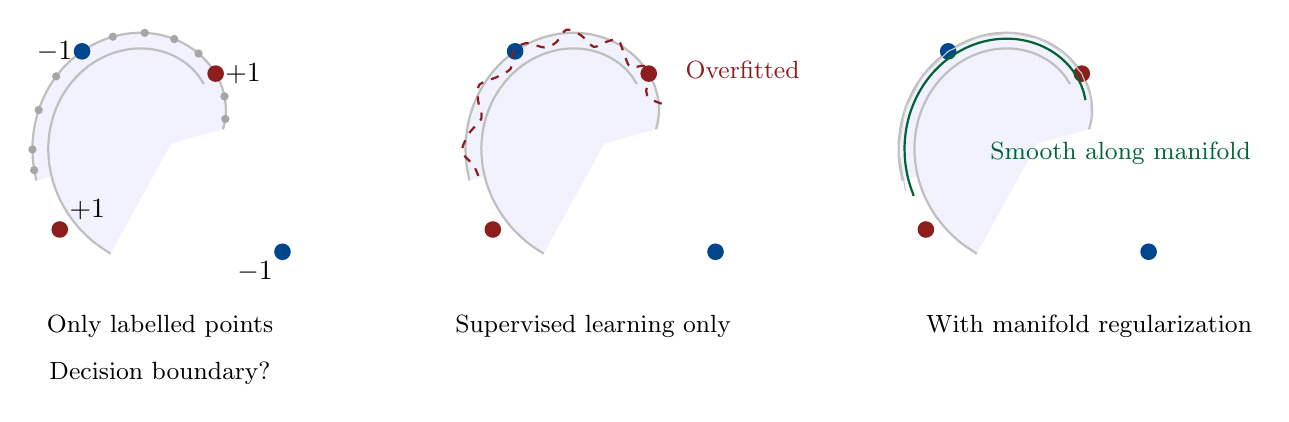
\begin{tikzpicture}[scale=1.0]
% Left: Swiss roll with labeled points only
\begin{scope}[xshift=-4cm]
  \draw[thick, gray!50, fill=blue!5]
    plot[domain=0:4.5, smooth]
    ({cos(deg(2*pi*\x/8))*(0.8+0.2*\x)},
     {sin(deg(2*pi*\x/8))*(0.8+0.2*\x)});
  \draw[thick, gray!50, fill=blue!5]
    plot[domain=0:4.5, smooth]
    ({cos(deg(2*pi*\x/8+0.8))*(0.8+0.2*\x)},
     {sin(deg(2*pi*\x/8+0.8))*(0.8+0.2*\x)});

  % Labeled points (few)
  \fill[manifoldred]
    ({cos(deg(2*pi*1/8))*(0.8+0.2*1)},
     {sin(deg(2*pi*1/8))*(0.8+0.2*1)})
    circle (3pt) node[right, black] {$+1$};
  \fill[manifoldblue]
    ({cos(deg(2*pi*3/8))*(0.8+0.2*3)},
     {sin(deg(2*pi*3/8))*(0.8+0.2*3)})
    circle (3pt) node[left, black] {$-1$};
  \fill[manifoldred]
    ({cos(deg(2*pi*5/8))*(0.8+0.2*5)},
     {sin(deg(2*pi*5/8))*(0.8+0.2*5)})
    circle (3pt) node[above right, black] {$+1$};
  \fill[manifoldblue]
    ({cos(deg(2*pi*7/8))*(0.8+0.2*7)},
     {sin(deg(2*pi*7/8))*(0.8+0.2*7)})
    circle (3pt) node[below left, black] {$-1$};

  % Unlabeled points (many, gray)
  \foreach \t in {0.2,0.6,1.4,1.8,2.2,2.6,3.4,3.8,4.2,4.4} {
    \fill[gray!70]
      ({cos(deg(2*pi*\t/8))*(0.8+0.2*\t)},
       {sin(deg(2*pi*\t/8))*(0.8+0.2*\t)})
      circle (1.5pt);
  }

  \node[font=\small] at (0, -2.5) {Only labelled points};
  \node[font=\small] at (0, -3.1) {Decision boundary?};
\end{scope}

% Middle: Pure supervised decision boundary
\begin{scope}[xshift=1.5cm]
  \draw[thick, gray!50, fill=blue!5]
    plot[domain=0:4.5, smooth]
    ({cos(deg(2*pi*\x/8))*(0.8+0.2*\x)},
     {sin(deg(2*pi*\x/8))*(0.8+0.2*\x)});
  \draw[thick, gray!50, fill=blue!5]
    plot[domain=0:4.5, smooth]
    ({cos(deg(2*pi*\x/8+0.8))*(0.8+0.2*\x)},
     {sin(deg(2*pi*\x/8+0.8))*(0.8+0.2*\x)});

  % Same labeled points
  \fill[manifoldred]
    ({cos(deg(2*pi*1/8))*(0.8+0.2*1)},
     {sin(deg(2*pi*1/8))*(0.8+0.2*1)}) circle (3pt);
  \fill[manifoldblue]
    ({cos(deg(2*pi*3/8))*(0.8+0.2*3)},
     {sin(deg(2*pi*3/8))*(0.8+0.2*3)}) circle (3pt);
  \fill[manifoldred]
    ({cos(deg(2*pi*5/8))*(0.8+0.2*5)},
     {sin(deg(2*pi*5/8))*(0.8+0.2*5)}) circle (3pt);
  \fill[manifoldblue]
    ({cos(deg(2*pi*7/8))*(0.8+0.2*7)},
     {sin(deg(2*pi*7/8))*(0.8+0.2*7)}) circle (3pt);

  % Supervised decision boundary (wiggly, overfitted)
  \draw[manifoldred, thick, dashed]
    plot[domain=0.2:4.3, smooth]
    ({cos(deg(2*pi*\x/8+0.2))*(0.8+0.2*\x+0.1*sin(deg(10*\x)))},
     {sin(deg(2*pi*\x/8+0.2))*(0.8+0.2*\x+0.1*sin(deg(10*\x)))});
  \node[font=\small, manifoldred] at (1.9, 0.75) {Overfitted};

  \node[font=\small] at (0, -2.5) {Supervised learning only};
\end{scope}

% Right: Manifold regularization
\begin{scope}[xshift=7cm]
  \draw[thick, gray!50, fill=blue!5]
    plot[domain=0:4.5, smooth]
    ({cos(deg(2*pi*\x/8))*(0.8+0.2*\x)},
     {sin(deg(2*pi*\x/8))*(0.8+0.2*\x)});
  \draw[thick, gray!50, fill=blue!5]
    plot[domain=0:4.5, smooth]
    ({cos(deg(2*pi*\x/8+0.8))*(0.8+0.2*\x)},
     {sin(deg(2*pi*\x/8+0.8))*(0.8+0.2*\x)});

  % Same labeled points
  \fill[manifoldred]
    ({cos(deg(2*pi*1/8))*(0.8+0.2*1)},
     {sin(deg(2*pi*1/8))*(0.8+0.2*1)}) circle (3pt);
  \fill[manifoldblue]
    ({cos(deg(2*pi*3/8))*(0.8+0.2*3)},
     {sin(deg(2*pi*3/8))*(0.8+0.2*3)}) circle (3pt);
  \fill[manifoldred]
    ({cos(deg(2*pi*5/8))*(0.8+0.2*5)},
     {sin(deg(2*pi*5/8))*(0.8+0.2*5)}) circle (3pt);
  \fill[manifoldblue]
    ({cos(deg(2*pi*7/8))*(0.8+0.2*7)},
     {sin(deg(2*pi*7/8))*(0.8+0.2*7)}) circle (3pt);

  % Graph edges connecting nearby points along the manifold
  \foreach \t in {0.2,0.6,1.0,1.4,1.8,2.2,2.6,3.0,3.4,3.8,4.2} {
    \pgfmathsetmacro{\next}{\t+0.4}
    \draw[gray!40, thin]
      ({cos(deg(2*pi*\t/8))*(0.8+0.2*\t)},
       {sin(deg(2*pi*\t/8))*(0.8+0.2*\t)}) --
      ({cos(deg(2*pi*\next/8))*(0.8+0.2*\next)},
       {sin(deg(2*pi*\next/8))*(0.8+0.2*\next)});
  }

  % Manifold-aware decision boundary
  \draw[manifoldgreen, thick]
    plot[domain=0.2:4.3, smooth]
    ({cos(deg(2*pi*\x/8+0.3))*(0.8+0.2*\x)},
     {sin(deg(2*pi*\x/8+0.3))*(0.8+0.2*\x)});
  \node[font=\small, manifoldgreen] at (1.2, -0.3) {Smooth along manifold};

  \node[font=\small] at (0.8, -2.5) {With manifold regularization};
\end{scope}
\end{tikzpicture}
\caption{Why unlabelled data matter. Left: Only four labelled
points on a Swiss roll manifold. Middle: A pure supervised
method overfits. Right: Manifold regularization uses graph
connections (grey edges) to enforce smoothness along the manifold.}
\label{semi-supervised-graphs:fig:manifold_motivation}
\end{figure}

To encode the geometry of the data we build a \emph{similarity graph} on all $n$ points: nodes are the points, edges join points that are close (the $k$ nearest neighbours, or all points within distance $\varepsilon$), and an edge carries a weight $A_{ij} > 0$, either $1$ or a Gaussian $\exp(-\norm{x_i - x_j}^2/2\sigma_g^2)$. By \cref{semi-supervised-graphs:thm:laplacian_quadratic}, the Laplacian $L = D - A$ of this graph satisfies, for the vector $\mathbf f$ of values of $f$ at the data points,
\[
\mathbf{f}^\top L \mathbf{f} = \frac{1}{2} \sum_{i,j=1}^n A_{ij}\bigl(f(x_i) - f(x_j)\bigr)^2 .
\]
The quadratic form is small when $f$ varies little across heavy edges, that is, along the data manifold as sampled by the graph.

\subsubsection*{The objective and the extended representer theorem}

We now combine two sources of information:

\begin{enumerate}[label=\emph{(\roman*)}]
  \item \textbf{Labelled data:} Supervised loss $\sum_{i=1}^l \ell(f(x_i), y_i)$.
  \item \textbf{Unlabelled data geometry:} Graph smoothness penalty
    $\mathbf{f}^\top L \mathbf{f}$.
\end{enumerate}

\begin{theorem}[Extended representer theorem]
\label{semi-supervised-graphs:thm:manifold_reg}
Let $\mathcal{H}_K$ be an RKHS with kernel $K$, and let $x_1,\ldots,x_n \in \mathcal{X}$
be all available data points, of which the first $l$ are labelled with
targets $y_1,\ldots,y_l \in \R$. Construct a graph over all $n$ points
with Laplacian $L$. Consider:
\begin{equation}
\label{semi-supervised-graphs:eq:manifold_reg}
\min_{f \in \mathcal{H}_K}\;
\underbrace{\frac{1}{l}\sum_{i=1}^{l}\ell(f(x_i), y_i)}_{\text{supervised loss}}
+ \underbrace{\gamma_A\norm{f}_{\mathcal{H}_K}^2}_{\text{ambient}}
+ \underbrace{\frac{\gamma_I}{n^2}\,\mathbf{f}^\top L\,\mathbf{f}}_{\text{intrinsic}}
\end{equation}
where $\mathbf{f} = (f(x_1), \ldots, f(x_n))^\top$ and
$\gamma_A, \gamma_I > 0$ are regularization parameters.

Then the minimizer admits the following representation:
\begin{equation}
\label{semi-supervised-graphs:eq:manifold_solution}
\boxed{f^*(x) = \sum_{i=1}^n \alpha_i^* K(x, x_i)
\quad \text{for some } \boldsymbol{\alpha}^* \in \R^n}
\end{equation}
\end{theorem}

\begin{intuition}[Two regularizers, two types of smoothness]
The two penalty terms encode complementary inductive biases:

\begin{itemize}
  \item \textbf{Ambient regularizer} ($\gamma_A\norm{f}_{\mathcal{H}_K}^2$): \\
  Forces $f$ to be smooth in the \emph{ambient space} $\R^d$. This is
  the standard RKHS penalty from \cref{rkhs:sec:representer}; for the linear
  kernel it is $\norm{w}^2$, as in ridge regression or the SVM.

  \item \textbf{Intrinsic regularizer} ($\gamma_I \mathbf{f}^\top L \mathbf{f}$): \\
  Forces $f$ to be smooth along the \emph{data manifold}. Two points
  connected by a high-weight edge are encouraged to have similar
  predictions, regardless of their Euclidean distance.
\end{itemize}

The ratio $\gamma_I / \gamma_A$ controls how much we trust the
unlabelled data geometry versus the supervised signal. When
$\gamma_I = 0$, we recover standard supervised kernel methods.
\end{intuition}

Why does the solution still have the form $\sum_{i=1}^n \alpha_i
K(\cdot, x_i)$, now using \emph{all} $n$ points? The proof is an
elegant extension of the classical representer theorem
(\cref{rkhs:thm:representer}).

\begin{proof}[Proof sketch]
Let $M = \operatorname{span}\{K(\cdot, x_1), \ldots, K(\cdot, x_n)\} \subseteq \mathcal{H}_K$.
Any $f \in \mathcal{H}_K$ decomposes as $f = f_\parallel + f_\perp$ with
$f_\parallel \in M$ and $f_\perp \in M^\perp$.

\smallskip
\emph{Step 1: the loss and intrinsic regularizer see only $f_\parallel$.}
\begin{itemize}
  \item By the reproducing property, $f(x_i) = \inner{f}{K(\cdot, x_i)}
    = f_\parallel(x_i)$ for each $i = 1,\ldots,n$. Hence the supervised
    loss depends only on $f_\parallel$.
  \item The vector $\mathbf{f} = (f(x_1),\ldots,f(x_n))^\top$ is determined
    entirely by $f_\parallel$, so $\mathbf{f}^\top L \mathbf{f}$ also
    depends only on $f_\parallel$.
\end{itemize}

\emph{Step 2: the ambient regularizer penalizes $f_\perp$ without
contributing to the other terms.}
By orthogonality, $\norm{f}_{\mathcal{H}_K}^2 = \norm{f_\parallel}_{\mathcal{H}_K}^2
+ \norm{f_\perp}_{\mathcal{H}_K}^2 \geq \norm{f_\parallel}_{\mathcal{H}_K}^2$.

\emph{Step 3: conclude.}
For any $f$, the objective $J(f) \geq J(f_\parallel)$ with equality
iff $f_\perp = 0$. Therefore the minimizer must lie in $M$, i.e.\
$f^* = \sum_{i=1}^n \alpha_i K(\cdot, x_i)$.
\end{proof}

\begin{remark}
The crucial difference from the classical representer theorem: the
intrinsic regularizer involves \emph{evaluations} $f(x_i)$ at
\emph{all} $n$ points, not just the labelled ones. This is why the
expansion now includes \emph{every} data point.
\end{remark}

\subsubsection*{Kernelization: the manifold regularization algorithm}

As in \cref{rkhs:sec:representer}, substitute
$f(x) = \sum_{j=1}^n \alpha_j K(x, x_j)$ into the objective.

\begin{align*}
\text{Prediction vector:} &\quad \mathbf{f} = \mathbf{K} \boldsymbol{\alpha}, \\
\text{Ambient regularizer:} &\quad \norm{f}_{\mathcal{H}_K}^2
  = \boldsymbol{\alpha}^\top \mathbf{K} \boldsymbol{\alpha}, \\
\text{Intrinsic regularizer:} &\quad \mathbf{f}^\top L \mathbf{f}
  = \boldsymbol{\alpha}^\top \mathbf{K} L \mathbf{K} \boldsymbol{\alpha}.
\end{align*}

\begin{theorem}[Kernelized manifold regularization]
\label{semi-supervised-graphs:thm:manifold_kernelized}
The manifold regularization problem~\eqref{semi-supervised-graphs:eq:manifold_reg} reduces to:
\begin{equation}
\label{semi-supervised-graphs:eq:manifold_kernelized}
\boxed{\min_{\boldsymbol{\alpha} \in \R^n}\;
\frac{1}{l}\sum_{i=1}^{l} \ell\bigl((\mathbf{K}\boldsymbol{\alpha})_i,\; y_i\bigr)
+ \gamma_A\,\boldsymbol{\alpha}^\top\mathbf{K}\boldsymbol{\alpha}
+ \frac{\gamma_I}{n^2}\,\boldsymbol{\alpha}^\top \mathbf{K}L\mathbf{K}\boldsymbol{\alpha}}
\end{equation}
This is convex for convex loss functions $\ell$ (e.g.\ squared loss,
hinge loss, logistic loss).
\end{theorem}

With the hinge loss this is the Laplacian SVM (LapSVM), with the squared loss Laplacian regularized least squares (LapRLS). Unlike label propagation, the result is a function on the whole input space, so it applies to new points (it is inductive).

\subsubsection*{Concrete example: two moons dataset}

For the squared loss, the kernelized problem \eqref{semi-supervised-graphs:eq:manifold_kernelized} is a quadratic in $\boldsymbol\alpha$. Let $\mathbf K_l$ be the $l\times n$ matrix of the rows of $\mathbf K$ that belong to labelled points, so that $(f(x_1), \ldots, f(x_l))^\top = \mathbf K_l\boldsymbol\alpha$. Setting the gradient of
\[
\frac{1}{l} \|\mathbf{K}_l \boldsymbol{\alpha} - \mathbf{y}\|^2
+ \gamma_A \boldsymbol{\alpha}^\top \mathbf{K} \boldsymbol{\alpha}
+ \frac{\gamma_I}{n^2} \boldsymbol{\alpha}^\top \mathbf{K}L\mathbf{K} \boldsymbol{\alpha}
\]
to zero gives the linear system of \emph{Laplacian regularized least squares} (LapRLS):
\begin{equation}
\left( \frac{1}{l} \mathbf{K}_l^\top \mathbf{K}_l + \gamma_A \mathbf{K}
+ \frac{\gamma_I}{n^2} \mathbf{K}L\mathbf{K} \right) \boldsymbol{\alpha}
= \frac{1}{l} \mathbf{K}_l^\top \mathbf{y}.
\label{semi-supervised-graphs:eq:laprls}
\end{equation}

\begin{example}[Two moons]
\label{semi-supervised-graphs:ex:manifold_two_moons}
We draw $n = 200$ points from the ``two moons'' distribution ($100$ per moon, Gaussian noise of standard deviation $0.08$; \texttt{make\_moons} of scikit-learn with seed $0$) and reveal the labels of only $l = 4$ points, two per moon. We use the Gaussian kernel with $\sigma = 0.5$, $\gamma_A = 0.01$, and a symmetrized $10$-nearest-neighbour graph with Gaussian weights ($\sigma_g = 0.5$). Solving \eqref{semi-supervised-graphs:eq:laprls} and classifying every point by the sign of $f^*$ gives the following accuracies on all $200$ points:
\begin{center}
\begin{tabular}{lcccc}
\toprule
$\gamma_I$ & $0$ & $1$ & $10^2$ & $10^4$ \\
\midrule
accuracy & $80.5\%$ & $81.0\%$ & $97.0\%$ & $100\%$ \\
\bottomrule
\end{tabular}
\end{center}
With $\gamma_I = 0$ the problem is kernel ridge regression on four points: the decision boundary is determined by distances in the plane and cuts through both moons (\cref{semi-supervised-graphs:fig:two_moons}, left). As $\gamma_I$ grows, the intrinsic penalty forces $f$ to be nearly constant along each moon, where the graph has many heavy edges, and the boundary moves into the low-density gap between them (right). The factor $1/n^2$ makes the intrinsic term small at this sample size; what matters is the effective weight $\gamma_I/n^2$, here $0.25$ for $\gamma_I = 10^4$.
\end{example}

\begin{figure}[ht]
\centering
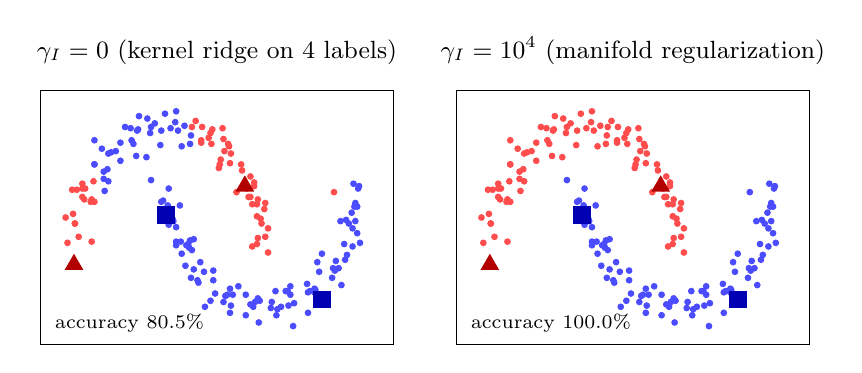
\begin{tikzpicture}
\begin{axis}[name=left,
  width=0.5\linewidth, height=4.8cm, title={$\gamma_I = 0$ (kernel ridge on 4 labels)}, title style={font=\small},
  xmin=-1.4, xmax=2.4, ymin=-0.8, ymax=1.3, xtick=\empty, ytick=\empty]
\addplot[only marks, mark=*, mark size=1pt, blue!70] coordinates {(1.63,-0.43) (-0.05,0.27) (1.77,-0.19) (1.90,-0.06) (0.89,-0.49) (1.14,-0.56) (-0.37,0.76) (0.22,-0.25) (1.81,-0.17) (1.26,-0.36) (-0.82,0.69) (0.30,-0.29) (-0.82,0.89) (1.96,0.01) (0.86,-0.47) (1.29,-0.32) (-0.25,1.07) (0.23,-0.02) (1.88,-0.10) (1.87,0.03) (0.12,-0.05) (0.12,0.84) (-0.26,0.75) (0.96,-0.44) (0.03,0.22) (1.89,0.23) (0.46,-0.19) (-0.08,0.39) (0.57,-0.45) (-0.40,0.86) (0.11,0.05) (1.55,-0.34) (-0.35,0.98) (-0.72,0.63) (0.16,-0.15) (0.91,-0.45) (-0.74,0.82) (0.36,-0.20) (2.04,0.04) (1.08,-0.50) (1.19,-0.49) (0.22,0.93) (-0.21,1.00) (0.29,-0.27) (1.75,-0.17) (1.09,-0.45) (-0.17,1.03) (1.50,-0.36) (0.08,0.97) (0.65,-0.48) (0.37,-0.49) (-0.21,0.56) (0.81,-0.39) (0.06,0.17) (0.73,-0.32) (2.01,0.12) (-0.10,0.97) (0.64,-0.54) (2.02,0.49) (0.02,0.24) (-0.34,1.09) (-0.36,0.97) (0.61,-0.39) (1.99,0.37) (1.99,0.22) (-0.67,0.78) (2.01,0.34) (1.78,-0.11) (1.74,-0.25) (0.46,-0.27) (0.06,0.05) (1.32,-0.65) (1.98,0.34) (0.06,1.13) (0.10,0.35) (-0.49,1.00) (1.56,-0.35) (0.21,0.86) (-0.59,0.80) (0.05,1.04) (-0.06,1.11) (1.48,-0.54) (1.96,0.16) (0.59,-0.40) (-0.67,0.55) (-0.05,0.31) (-0.00,0.99) (-0.10,0.38) (-0.82,0.69) (0.21,0.06) (1.29,-0.39) (1.97,0.53) (-0.54,0.72) (0.25,-0.18) (1.24,-0.36) (1.58,-0.12) (1.13,-0.36) (2.03,0.51) (0.06,0.02) (-0.02,0.49) (-0.43,0.99) (-0.42,0.89) (0.25,0.07) (1.33,-0.46) (-0.02,0.19) (0.48,-0.38) (1.68,-0.42) (0.64,-0.34) (-0.22,0.95) (1.27,-0.48) (0.32,-0.12) (0.19,0.03) (1.15,-0.51) (1.47,-0.30) (0.43,-0.44) (1.63,-0.05) (0.67,-0.39) (1.55,-0.37) (0.95,-0.62) (-0.71,0.47) (0.17,0.02) (0.94,-0.42) (-0.68,0.65) (-0.72,0.57) (1.48,-0.37) (1.92,0.20) (1.84,-0.31) (1.95,0.29) (-0.11,0.85) (0.81,-0.56) (-0.64,0.79) (-0.03,0.35) (-0.54,0.87) (1.83,0.22) (0.20,-0.00) (0.15,1.01) (1.60,-0.20)};
\addplot[only marks, mark=*, mark size=1pt, red!70] coordinates {(0.80,0.51) (-1.04,-0.14) (0.97,0.24) (0.88,0.36) (0.98,0.20) (0.57,0.90) (0.33,0.87) (0.23,1.00) (0.90,0.54) (0.76,0.69) (0.94,0.08) (-0.83,0.55) (0.64,0.70) (1.05,0.16) (-0.85,0.05) (0.77,0.64) (0.53,0.69) (-1.03,0.20) (0.90,0.51) (-1.13,0.25) (-0.95,0.49) (-1.01,0.48) (-0.95,0.42) (0.94,0.40) (0.58,0.80) (0.93,0.03) (0.41,0.91) (1.02,0.37) (-1.05,0.28) (1.05,-0.04) (-0.85,0.40) (-0.99,0.09) (-0.82,0.38) (0.93,0.36) (0.52,0.66) (0.71,0.46) (0.86,0.59) (0.88,0.01) (1.01,0.32) (-1.06,0.48) (-1.03,0.20) (0.86,0.42) (0.45,0.98) (1.02,0.09) (0.27,1.05) (0.84,0.42) (0.33,0.89) (0.56,0.99) (0.65,0.78) (0.63,0.84) (0.44,0.86) (0.62,0.86) (-1.11,0.04) (-0.95,0.53) (1.76,0.46) (0.54,0.73) (-0.92,0.49) (0.34,1.00) (-0.86,0.38) (-0.93,0.40) (0.43,0.95) (0.82,0.49) (0.93,0.26)};
\addplot[only marks, mark=square*, mark size=3pt, blue!70!black] coordinates {(1.63,-0.43) (-0.05,0.27)};
\addplot[only marks, mark=triangle*, mark size=3.5pt, red!70!black] coordinates {(0.80,0.51) (-1.04,-0.14)};
\node[font=\scriptsize, anchor=south west] at (axis cs:-1.35,-0.78) {accuracy 80.5\%};
\end{axis}
\begin{axis}[name=right,at={(left.east)}, anchor=west, xshift=0.8cm,
  width=0.5\linewidth, height=4.8cm, title={$\gamma_I = 10^4$ (manifold regularization)}, title style={font=\small},
  xmin=-1.4, xmax=2.4, ymin=-0.8, ymax=1.3, xtick=\empty, ytick=\empty]
\addplot[only marks, mark=*, mark size=1pt, blue!70] coordinates {(1.63,-0.43) (-0.05,0.27) (1.77,-0.19) (1.90,-0.06) (0.89,-0.49) (1.14,-0.56) (0.22,-0.25) (1.81,-0.17) (1.26,-0.36) (0.30,-0.29) (1.96,0.01) (0.86,-0.47) (1.29,-0.32) (0.23,-0.02) (1.88,-0.10) (1.87,0.03) (0.12,-0.05) (0.96,-0.44) (0.03,0.22) (1.89,0.23) (0.46,-0.19) (-0.08,0.39) (0.57,-0.45) (0.11,0.05) (1.55,-0.34) (0.16,-0.15) (0.91,-0.45) (0.36,-0.20) (2.04,0.04) (1.08,-0.50) (1.19,-0.49) (0.29,-0.27) (1.75,-0.17) (1.09,-0.45) (1.50,-0.36) (0.65,-0.48) (0.37,-0.49) (-0.21,0.56) (0.81,-0.39) (0.06,0.17) (0.73,-0.32) (2.01,0.12) (0.64,-0.54) (2.02,0.49) (0.02,0.24) (0.61,-0.39) (1.99,0.37) (1.99,0.22) (2.01,0.34) (1.78,-0.11) (1.74,-0.25) (0.46,-0.27) (0.06,0.05) (1.32,-0.65) (1.98,0.34) (0.10,0.35) (1.56,-0.35) (1.48,-0.54) (1.96,0.16) (0.59,-0.40) (-0.05,0.31) (-0.10,0.38) (0.21,0.06) (1.29,-0.39) (1.97,0.53) (0.25,-0.18) (1.24,-0.36) (1.58,-0.12) (1.13,-0.36) (2.03,0.51) (0.06,0.02) (-0.02,0.49) (0.25,0.07) (1.33,-0.46) (-0.02,0.19) (0.48,-0.38) (1.68,-0.42) (0.64,-0.34) (1.27,-0.48) (0.32,-0.12) (0.19,0.03) (1.15,-0.51) (1.47,-0.30) (0.43,-0.44) (1.63,-0.05) (0.67,-0.39) (1.55,-0.37) (0.95,-0.62) (0.17,0.02) (0.94,-0.42) (1.76,0.46) (1.48,-0.37) (1.92,0.20) (1.84,-0.31) (1.95,0.29) (0.81,-0.56) (-0.03,0.35) (1.83,0.22) (0.20,-0.00) (1.60,-0.20)};
\addplot[only marks, mark=*, mark size=1pt, red!70] coordinates {(0.80,0.51) (-1.04,-0.14) (0.97,0.24) (0.88,0.36) (-0.37,0.76) (-0.82,0.69) (0.98,0.20) (0.57,0.90) (0.33,0.87) (-0.82,0.89) (0.23,1.00) (-0.25,1.07) (0.12,0.84) (0.90,0.54) (-0.26,0.75) (0.76,0.69) (0.94,0.08) (-0.83,0.55) (-0.40,0.86) (0.64,0.70) (-0.35,0.98) (1.05,0.16) (-0.72,0.63) (-0.74,0.82) (-0.85,0.05) (0.77,0.64) (0.53,0.69) (0.22,0.93) (-0.21,1.00) (-1.03,0.20) (0.90,0.51) (-1.13,0.25) (-0.17,1.03) (0.08,0.97) (-0.95,0.49) (-1.01,0.48) (-0.95,0.42) (0.94,0.40) (0.58,0.80) (-0.10,0.97) (-0.34,1.09) (0.93,0.03) (-0.36,0.97) (0.41,0.91) (1.02,0.37) (-0.67,0.78) (-1.05,0.28) (0.06,1.13) (1.05,-0.04) (-0.85,0.40) (-0.99,0.09) (-0.49,1.00) (0.21,0.86) (-0.59,0.80) (0.05,1.04) (-0.06,1.11) (-0.82,0.38) (0.93,0.36) (0.52,0.66) (0.71,0.46) (0.86,0.59) (-0.67,0.55) (-0.00,0.99) (-0.82,0.69) (0.88,0.01) (1.01,0.32) (-0.54,0.72) (-1.06,0.48) (-1.03,0.20) (0.86,0.42) (0.45,0.98) (-0.43,0.99) (-0.42,0.89) (1.02,0.09) (0.27,1.05) (0.84,0.42) (0.33,0.89) (-0.22,0.95) (0.56,0.99) (0.65,0.78) (0.63,0.84) (0.44,0.86) (0.62,0.86) (-1.11,0.04) (-0.95,0.53) (-0.71,0.47) (-0.68,0.65) (-0.72,0.57) (0.54,0.73) (-0.92,0.49) (0.34,1.00) (-0.11,0.85) (-0.86,0.38) (-0.64,0.79) (-0.93,0.40) (0.43,0.95) (0.82,0.49) (0.93,0.26) (-0.54,0.87) (0.15,1.01)};
\addplot[only marks, mark=square*, mark size=3pt, blue!70!black] coordinates {(1.63,-0.43) (-0.05,0.27)};
\addplot[only marks, mark=triangle*, mark size=3.5pt, red!70!black] coordinates {(0.80,0.51) (-1.04,-0.14)};
\node[font=\scriptsize, anchor=south west] at (axis cs:-1.35,-0.78) {accuracy 100.0\%};
\end{axis}
\end{tikzpicture}
\caption{Manifold regularization on the two moons (computed). Points are coloured by the sign of the learned $f^*$; the four labelled points are drawn as large squares ($+1$) and triangles ($-1$). Left: without the intrinsic penalty the boundary ignores the shape of the data. Right: with it the two moons are separated exactly.}
\label{semi-supervised-graphs:fig:two_moons}
\end{figure}

\subsubsection*{Practical considerations}

\begin{enumerate}[label=\emph{\arabic*.}]
  \item \textbf{Choosing the graph.}
  \begin{itemize}
    \item $k$-NN graph: common choices $k = 5$--$20$.
    \item $\varepsilon$-ball graph: connect points within distance $\varepsilon$.
    \item Edge weights: binary, Gaussian, or cosine similarity.
  \end{itemize}

  \item \textbf{Normalization.} The factor $1/n^2$ ensures consistent
    scaling as $n$ grows. Often $L$ is replaced by the normalized
    Laplacian $\mathcal L_{\mathrm{sym}} = I - D^{-1/2}AD^{-1/2}$.

  \item \textbf{Computational cost.}
  \begin{itemize}
    \item Computing $\mathbf{K}$ is $O(n^2 d)$, constructing the $k$-NN graph
      is $O(n^2 d)$.
    \item Solving the linear system is $O(n^3)$ --- the main bottleneck.
    \item For large $n$, use Nystr\"om approximation or iterative solvers.
  \end{itemize}

  \item \textbf{Relation to other methods.} Neural graph learning
    (\cref{semi-supervised-graphs:subsec:neural_graph}) applies the same penalty
    to a neural network; graph neural networks (\cref{semi-supervised-graphs:sec:gnn})
    are the modern deep learning analogue.
\end{enumerate}

\subsubsection*{Connection to Mercer's theorem}

The two regularizers can be understood through Mercer's theorem (\cref{rkhs:thm:mercer}), which writes $f = \sum_k a_k e_k$ in the eigenfunctions $e_k$ of the kernel, with eigenvalues $\lambda_k$:

\begin{itemize}
  \item The \emph{ambient regularizer} $\gamma_A \norm{f}_{\mathcal{H}_K}^2
    = \gamma_A \sum_k a_k^2/\lambda_k$ penalizes high-frequency
    components in the eigenbasis of $K$.
  \item The \emph{intrinsic regularizer} $\gamma_I \mathbf{f}^\top
    L \mathbf{f}$ penalizes variations along the data manifold.
\end{itemize}

The two penalties are measured in different spectral bases: that of the integral operator of $K$ on the ambient space, and that of $L$ on the sample. They agree only when the kernel already reflects the manifold, for instance when $K$ is itself built from the graph (as for the diffusion kernel $e^{-tL}$).

\subsubsection*{Summary: why manifold regularization works}

\begin{keyidea}[The manifold regularization recipe]
\begin{enumerate}
  \item \textbf{Start with a kernel} $K$ that encodes ambient smoothness.
  \item \textbf{Build a graph} from \emph{all} data points to capture
    manifold geometry.
  \item \textbf{Add the graph Laplacian penalty} $\mathbf{f}^\top L
    \mathbf{f}$ to enforce smoothness along the manifold.
  \item \textbf{Solve} the kernelized problem ($\boldsymbol{\alpha} \in \R^n$).
  \item \textbf{Predict} using $f(x) = \sum_{i=1}^n \alpha_i K(x, x_i)$.
\end{enumerate}

The magic: unlabelled data enter through:
\begin{enumerate}[label=(\alph*)]
  \item The representation $f(x) = \sum_{i=1}^n \alpha_i K(x, x_i)$
    includes \emph{all} points.
  \item The graph Laplacian $L$ is constructed from \emph{all}
    points.
\end{enumerate}
\end{keyidea}

\subsection{Neural graph learning}
\label{semi-supervised-graphs:subsec:neural_graph}

LapSVM searches over a rich kernel space but ultimately produces a linear
decision function in the RKHS feature map. In many applications, the
relationship between node features and labels is highly nonlinear, and one
would prefer to learn the feature representation end-to-end. Neural graph
learning (Bui, Ravi and Ramavajjala, \emph{Neural Graph Learning: Training Neural Networks Using Graphs}, 2018) applies the same graph regularization idea to deep
networks: the model $f_\theta$ is an arbitrary feedforward neural network, and
the graph smoothness penalty is applied to its intermediate representations.

\subsubsection*{The objective}

Let $f_\theta: \R^d \to \R^C$ be a $K$-layer neural network with hidden
representations $h_\theta^{(k)}(x) \in \R^{d_k}$ at layer $k$ (where
$h_\theta^{(0)}(x) = x$ and $h_\theta^{(K)}(x) = f_\theta(x)$). The neural
graph learning objective penalizes disagreement between connected nodes at
\emph{every} layer:
\begin{equation}
\label{semi-supervised-graphs:eq:neural_graph}
\mathcal{L}(\theta) = \underbrace{\sum_{i \in \mathcal{V}_L}
\ell(f_\theta(x_i), y_i)}_{\text{supervised loss}} +
\sum_{k=1}^K \lambda_k
\underbrace{\sum_{i,j}A_{ij}\|h_\theta^{(k)}(x_i) -
h_\theta^{(k)}(x_j)\|^2}_{= \,2\,\tr(H^{(k)\top} L\, H^{(k)})}
\end{equation}
where $\lambda_k > 0$ is the regularization strength at layer $k$, and
$H^{(k)} \in \R^{n \times d_k}$ is the matrix stacking all nodes' layer-$k$
representations. By \cref{semi-supervised-graphs:rem:trace_form} (applied column by column to
each layer), each smoothness term equals $2\,\tr(H^{(k)\top} L H^{(k)})$.

\subsubsection*{Why penalize every layer?}

Penalizing only the output layer (as in \cref{semi-supervised-graphs:def:graph_reg}) ensures
that the final predictions are smooth, but intermediate representations may
still be arbitrarily rough. Regularizing every hidden layer encourages the
network to build \emph{graph-consistent internal representations}: nodes that
are connected and should share a label are nudged towards similar activations at
every depth. This acts as a form of deep data augmentation using the graph
structure, and empirically leads to better generalization when labelled data is
scarce.

The per-layer weights $\lambda_k$ offer flexibility: setting $\lambda_k = 0$
for $k < K$ and $\lambda_K = \lambda$ recovers the single-output penalty of
\cref{semi-supervised-graphs:def:graph_reg}. In practice, deeper layers tend to benefit
from stronger regularization because they operate in higher-level representation
spaces where graph homophily is more meaningful.

\subsubsection*{Gradient computation}

Training proceeds by standard backpropagation. The gradient of the smoothness
term at layer $k$ with respect to the parameters $\theta$ is:
\[
\frac{\partial}{\partial \theta}\,\tr(H^{(k)\top} L H^{(k)})
= 2\,\frac{\partial H^{(k)}}{\partial \theta}^\top L H^{(k)},
\]
where $\partial H^{(k)}/\partial \theta$ is computed by the chain rule through
layers $1, \ldots, k$. Concretely, the ``signal'' backpropagated from the
smoothness term at layer $k$ is $2L H^{(k)} \in \R^{n \times d_k}$: it is the
Laplacian applied to the layer-$k$ representations, pushing each node's
representation towards the weighted average of its neighbours'.

\subsubsection*{Key distinction from GNNs}

\begin{pitfall}
In neural graph learning, the graph appears only in the \emph{loss function}
during training. At inference time, $f_\theta$ is a standard feedforward
network: a new node $x_{\text{new}}$ is classified by evaluating
$f_\theta(x_{\text{new}})$ alone, with no knowledge of the graph required.

Graph neural networks (\cref{semi-supervised-graphs:sec:gnn}), by contrast, build graph
aggregation directly into the \emph{architecture}: the forward pass itself
mixes information across neighbours, so the graph must be available at inference
time. This distinction has practical consequences summarized in the table below.
\end{pitfall}

\begin{center}
\small
\resizebox{\linewidth}{!}{%
\begin{tabular}{lcc}
\toprule
& Neural Graph Learning & GNN \\
\midrule
Graph used at training    & Yes (in loss)         & Yes (in forward pass) \\
Graph used at inference   & No                    & Yes \\
New nodes (inductive)     & Yes, trivially        & Yes, if the new node's neighbourhood is known \\
Over-smoothing risk       & Low (graph in loss only) & High (many layers) \\
Representational power    & Limited (no graph aggregation) & High \\
\bottomrule
\end{tabular}%
}
\end{center}

\section{Semi-supervised graph neural networks}
\label{semi-supervised-graphs:sec:gnn}

Graph regularization (\cref{semi-supervised-graphs:sec:reg}) uses the graph in the
\emph{loss function} but not in the model itself: each node is processed
independently by $f_\theta$. Graph Neural Networks (GNNs) go further --- they
build graph structure directly into the \emph{architecture}, allowing each
node to aggregate information from its neighbours as part of the forward pass.

\subsection{GNN layers}

GNN layers are instances of message passing (Gilmer et al., \emph{Neural Message Passing for Quantum Chemistry}, 2017), derived and compared in \cref{ch:dft-to-gnn}: after $K$ layers the representation $h_v^{(K)}$ of node $v$ depends on its $K$-hop neighbourhood. We use three of them.
\begin{itemize}
\item \textbf{GCN} (Kipf and Welling, \emph{Semi-Supervised Classification with Graph Convolutional Networks}, 2017): $H^{(k+1)} = \sigma(\hat AH^{(k)}W^{(k)})$ with $\hat A = \tilde D^{-1/2}\tilde A\tilde D^{-1/2}$, $\tilde A = A + I$; per node, $h_v^{(k+1)} = \sigma\bigl(\sum_{u\in\mathcal N(v)\cup\{v\}}(\tilde d_v\tilde d_u)^{-1/2}h_u^{(k)}W^{(k)}\bigr)$ with $\tilde d_v = d_v + 1$. It is the first-order simplification of a Chebyshev spectral filter (\cref{dft-to-gnn:sec:gcn}). The self-loops keep the node's own features and keep the eigenvalues of $\hat A$ in $(-1, 1]$, away from $-1$ (\cref{dft-to-gnn:exr:4}), which avoids the numerical instability of repeated multiplication by $I + D^{-1/2}AD^{-1/2}$, whose spectrum lies in $[0, 2]$.
\item \textbf{GraphSAGE} (Hamilton, Ying and Leskovec, \emph{Inductive Representation Learning on Large Graphs}, 2017) aggregates a \emph{sampled} fixed-size set of neighbours and concatenates the result with the node's own representation, $h_v^{(k)} = \sigma(W^{(k)}[h_v^{(k-1)}\,\|\,\mathrm{AGG}(\{h_u^{(k-1)}: u\in\mathcal S_k(\mathcal N(v))\})])$. Sampling bounds the cost per node and allows mini-batch training on very large graphs.
\item \textbf{GAT} (Veličković et al., \emph{Graph Attention Networks}, 2018) replaces the fixed GCN weights $(\tilde d_v\tilde d_u)^{-1/2}$, which depend only on degrees, by attention coefficients $\alpha_{vu}$ computed from the features of both endpoints, with several heads in parallel.
\end{itemize}

\begin{example}[One GCN layer on a triangle]
Triangle ($K_3$) with $H^{(0)} = \bigl(\begin{smallmatrix}1&0\\0&1\\1&1
\end{smallmatrix}\bigr)$. All $\tilde{d}_i = 3$, so $\hat{A} = \frac{1}{3}
\mathbf{1}\mathbf{1}^\top$. With $W^{(0)}=I$:
$\hat{A}H^{(0)} = \frac{1}{3}\bigl(\begin{smallmatrix}2&2\\2&2\\2&2
\end{smallmatrix}\bigr)$. All representations become identical
$(2/3,2/3)$ --- \emph{over-smoothing} in a single layer.
\end{example}

\subsection{Semi-supervised training}

The training loss is computed only on labelled nodes:
$\mathcal{L} = -\sum_{i \in \mathcal{V}_L}\sum_c Y_{ic}\log Z_{ic}$
where $Z = \softmax(\hat{A}\,\mathrm{ReLU}(\hat{A}XW^{(1)})\,W^{(2)})$
(a 2-layer GCN).

How do unlabelled nodes help, if the loss only involves labelled ones? The
answer lies in the forward pass: $\hat{A}H^{(k)}$ averages each node's features
with its neighbours'. When computing the representation of a labelled node $v_i$,
the GCN aggregates features from $v_i$'s unlabelled neighbours. So unlabelled
nodes contribute their feature information to the labelled nodes' representations,
and the gradients from labelled nodes propagate back through these aggregation
steps to update the shared weights $W^{(k)}$. This is a form of
\emph{transductive} semi-supervised learning: the unlabelled nodes are known at
training time and participate in every forward pass.

\begin{keyidea}
\emph{How unlabelled nodes get labelled: two distinct phases.}

\emph{Training phase:}
\begin{itemize}
    \item Loss computed \emph{only} on labelled nodes:
          $\mathcal{L} = -\sum_{i \in \mathcal{V}_L}\sum_c Y_{ic}\log Z_{ic}$.
    \item Unlabelled nodes appear in the \emph{forward pass} because
          $\hat{A}H^{(k)}$ aggregates each node's features with its neighbours'.
    \item When computing $Z_i$ for a \emph{labelled} node $i$, we aggregate
          features from its \emph{unlabelled} neighbours.
    \item Gradients from labelled nodes flow \emph{through} these unlabelled
          nodes' features during backpropagation, updating the shared weight
          matrices $W^{(k)}$.
    \item Unlabelled nodes themselves receive \emph{no direct gradient signal}
          and no loss is computed on their predictions during training.
\end{itemize}

\emph{Inference phase:}
\begin{itemize}
    \item After training completes, perform \emph{one} additional forward pass on
          \emph{all nodes} using the learned weights.
    \item For each unlabelled node $i \in \mathcal{V}_U$, take
          $\hat{y}_i = \argmax_c Z_{ic}$.
    \item \textbf{This is the first and only time unlabelled nodes receive
          predicted labels.}
\end{itemize}

Thus, unlabelled nodes are \emph{never labelled during training}. They serve as
``bridges'' that propagate information between labelled nodes and help learn
better feature extractors.
\end{keyidea}

\begin{pitfall}
\emph{Common misconception:} ``GCNs are trained to predict labels for unlabelled
nodes''. This is false. GCNs are trained to predict labels for \emph{labelled}
nodes. Unlabelled nodes are only used to compute better representations of
labelled nodes. The unlabelled node predictions are a \emph{byproduct} of this
process, not the training objective.
\end{pitfall}

\subsection{Over-smoothing}

\begin{pitfall}
For the propagation alone (no weights or nonlinearities), $\hat{A}^K H^{(0)}$ converges as $K \to \infty$ to a rank-1
matrix (Li, Han and Wu, \emph{Deeper Insights into Graph Convolutional Networks for Semi-Supervised Learning}, 2018): all node representations become indistinguishable.
Practical remedy: use 2--3 layers. For long-range dependencies:
JKNet (Xu et al., 2018), DropEdge (Rong et al., 2020),
PairNorm (Zhao and Akoglu, 2020), or graph transformers (Ying et al., 2021).
\end{pitfall}


%---------------------------------------------------------------------
\section{Self-supervised pretraining for GNNs}
\label{semi-supervised-graphs:sec:mlp}

The GNNs of \cref{semi-supervised-graphs:sec:gnn} are trained \emph{end-to-end} on the
semi-supervised task: they minimize a loss on the few labelled nodes while using
graph structure in their forward pass. But training from a random initialization
with only a handful of labels can be brittle --- the model may overfit to the few
labels or learn poor representations of the graph structure.

\emph{Self-supervised pretraining} addresses this by first training the GNN
on an auxiliary task that requires \emph{no labels at all}, then fine-tuning
on the downstream semi-supervised task. The idea, borrowed from masked language
modelling in NLP (BERT), is to hide part of the input and train the model to
reconstruct it from the remaining context.

\begin{keyidea}[Masked prediction pretraining]
\emph{Masked prediction pretraining (general scheme):}
\begin{enumerate}
    \item Randomly select a subset $\mathcal{M} \subset V$ of nodes.
    \item Hide some of their information (features, edges, or --- when
          available --- labels).
    \item Train a GNN to reconstruct the hidden information from the
          remaining graph context.
    \item Fine-tune the pretrained GNN on the downstream semi-supervised task.
\end{enumerate}
\end{keyidea}

\subsection{What can be masked?}

Three types of information can be masked during pretraining, each providing a
different learning signal.

\emph{Feature masking} (requires no labels). Replace feature vectors $x_i$
with a zero or learnable \texttt{[MASK]} vector for $i \in \mathcal{M}$, and
train the GNN to reconstruct $x_i$ from the unmasked neighbours. This teaches
the model to aggregate neighbourhood information --- exactly the skill needed for
message passing. Feature masking is the most widely applicable variant because
it requires no labels at all.

\emph{Edge masking} (requires no labels). Remove edges and train the model
to predict which edges exist (link prediction). This teaches the model the
graph's topology.

\emph{Label masking} (requires a large labelled dataset). Hide known labels
and predict them from the graph context. This provides the strongest signal
because it directly trains the model to propagate class information. However,
it requires that labels are available for \emph{most} nodes during
pretraining --- a much stronger assumption than the standard semi-supervised
setting.

\begin{pitfall}
\emph{When does label masking apply?} In the standard semi-supervised
setting, we have very few labels ($l \ll n$). Masking some of these
would further reduce supervision. Label masking is most useful when:
(a) a large fully labelled auxiliary graph is available (e.g.\ pretrain on a
large annotated citation network, then fine-tune on a smaller one), or
(b) labels come from a cheap proxy (e.g.\ automatically extracted
categories). Feature masking, by contrast, applies in \emph{any} setting.
\end{pitfall}

\subsection{Illustration: feature masking vs.\ label masking}

\begin{figure}[ht]
\centering
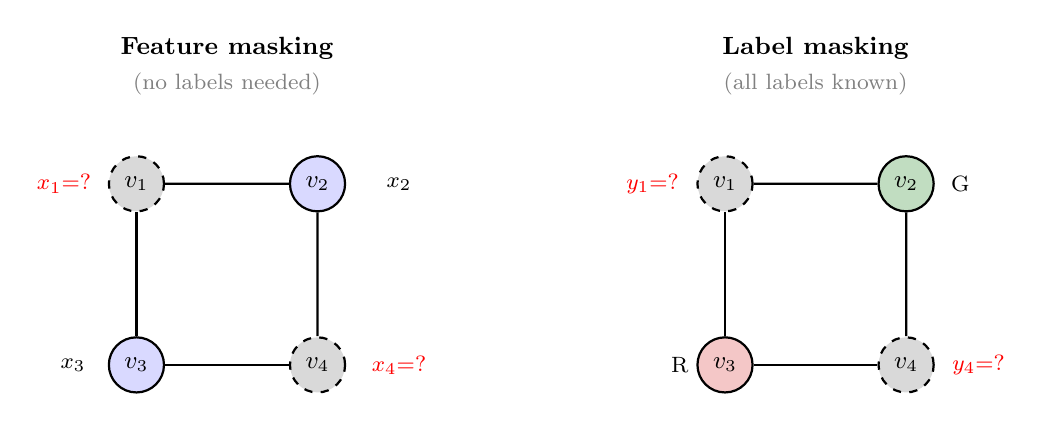
\begin{tikzpicture}[scale=1.15,
    node/.style={circle, draw, thick, minimum size=0.7cm, font=\small},
    masked/.style={circle, draw, thick, minimum size=0.7cm, font=\small,
      fill=gray!30, dashed}]

    % ---- LEFT: Feature masking (no labels needed) ----
    \begin{scope}[xshift=0cm]
        \node[draw=none, font=\small\bfseries] at (1,3.5)
          {Feature masking};
        \node[draw=none, font=\footnotesize, text=gray] at (1,3.1)
          {(no labels needed)};

        \node[masked] (a1) at (0,2) {$v_1$};
        \node[node, fill=blue!15] (a2) at (2,2) {$v_2$};
        \node[node, fill=blue!15] (a3) at (0,0) {$v_3$};
        \node[masked] (a4) at (2,0) {$v_4$};

        \draw[thick] (a1)--(a2); \draw[thick] (a1)--(a3);
        \draw[thick] (a2)--(a4); \draw[thick] (a3)--(a4);

        \node[draw=none, font=\footnotesize, text=red] at (-0.8,2) {$x_1{=}$?};
        \node[draw=none, font=\footnotesize] at (2.9,2) {$x_2$};
        \node[draw=none, font=\footnotesize] at (-0.7,0) {$x_3$};
        \node[draw=none, font=\footnotesize, text=red] at (2.9,0) {$x_4{=}$?};
    \end{scope}

    % ---- RIGHT: Label masking (fully labelled pretraining data) ----
    \begin{scope}[xshift=6.5cm]
        \node[draw=none, font=\small\bfseries] at (1,3.5)
          {Label masking};
        \node[draw=none, font=\footnotesize, text=gray] at (1,3.1)
          {(all labels known)};

        \node[masked] (b1) at (0,2) {$v_1$};
        \node[node, fill=labeledgreen!30] (b2) at (2,2) {$v_2$};
        \node[node, fill=labeledred!30] (b3) at (0,0) {$v_3$};
        \node[masked] (b4) at (2,0) {$v_4$};

        \draw[thick] (b1)--(b2); \draw[thick] (b1)--(b3);
        \draw[thick] (b2)--(b4); \draw[thick] (b3)--(b4);

        \node[draw=none, font=\footnotesize, text=red] at (-0.8,2) {$y_1{=}$?};
        \node[draw=none, font=\footnotesize] at (2.6,2) {G};
        \node[draw=none, font=\footnotesize] at (-0.5,0) {R};
        \node[draw=none, font=\footnotesize, text=red] at (2.8,0) {$y_4{=}$?};
    \end{scope}
\end{tikzpicture}
\caption{Two variants of masked pretraining. Left: feature masking hides
  $x_1, x_4$ and trains the GNN to reconstruct them (no labels needed).
  Right: label masking hides $y_1, y_4$ and trains the GNN to predict them
  (requires a fully labelled graph for pretraining). Grey dashed nodes are
  masked; the model must predict the ``?'' values from the remaining context.}
\label{semi-supervised-graphs:fig:masked_pretraining}
\end{figure}

\subsection{Mathematical formulation}

Let $\mathcal{M} \subset V$ be a random mask with ratio
$p = |\mathcal{M}|/n$ (typically $0.15$--$0.30$).

\paragraph{Feature masking objective.} Define the masked feature matrix
$\tilde{X}$ with $\tilde{X}_i = \mathbf{0}$ for $i \in \mathcal{M}$ and
$\tilde{X}_i = X_i$ otherwise. The pretraining loss is:
\begin{equation}
\label{semi-supervised-graphs:eq:feature_mask}
\mathcal{L}_{\text{feat}}(\theta) = \sum_{i \in \mathcal{M}}
  \|f_\theta(G, \tilde{X})_i - X_i\|^2
\end{equation}
To predict $X_i$, the GNN must aggregate information from $v_i$'s unmasked
neighbours via message passing --- exactly the skill needed for downstream tasks.

\emph{Label masking objective} (when a fully labelled pretraining graph is
available). Define $\tilde{Y}$ with $\tilde{Y}_i = \mathbf{0}$ for
$i \in \mathcal{M}$ and $\tilde{Y}_i = Y_i$ otherwise. The GNN receives
both features $X$ and unmasked labels $\tilde{Y}$ as input:
\begin{equation}
\label{semi-supervised-graphs:eq:label_mask}
\mathcal{L}_{\text{label}}(\theta) = -\sum_{i \in \mathcal{M}} \sum_{c=1}^C
  Y_{ic}\,\log\bigl(f_\theta(G, X, \tilde{Y})_i\bigr)_c
\end{equation}
The unmasked labels are provided as input because we want the model to learn
how to \emph{propagate} label information across the graph --- given some labels,
predict the rest. This directly simulates the semi-supervised scenario.

\subsection{The GPT-GNN framework}

GPT-GNN (Hu et al., \emph{GPT-GNN: Generative Pre-Training of Graph Neural Networks}, 2020) pretrains by generating masked node attributes and edges, which are the first two objectives below; label masking is used instead in methods that feed partial labels to the network, such as the unified message-passing model of Shi et al.\ (\emph{Masked Label Prediction}, 2021). A combined objective reads
\begin{equation}
\mathcal{L}_{\text{GPT-GNN}} =
  \underbrace{\mathcal{L}_{\text{feat}}}_{\substack{\text{reconstruct}\\\text{masked features}}}
  + \underbrace{\mathcal{L}_{\text{edge}}}_{\substack{\text{predict}\\\text{masked edges}}}
  + \lambda\underbrace{\mathcal{L}_{\text{label}}}_{\substack{\text{predict}\\\text{masked labels}}}
\end{equation}
with weights chosen by validation ($\lambda = 0$ when no pretraining labels exist). Each objective teaches a different skill: feature reconstruction teaches neighbourhood aggregation, edge prediction teaches the topology, and label prediction teaches class propagation.

\subsection{Why pretraining helps: intuition}

A randomly initialized GNN must simultaneously learn two things from the few
labelled nodes: (i) \emph{how} to aggregate neighbourhood information
(the ``mechanics'' of message passing), and (ii) \emph{which} aggregated
patterns correspond to which classes. Pretraining separates these: the model
first learns (i) from the self-supervised task (which uses no labels), then
only needs to learn (ii) from the few downstream labels. This is easier
because the representation is already informative.

This argument is heuristic: whether pretraining helps depends on how well the pretext task matches the downstream one, and negative transfer is observed when it does not.

\subsection{Practical implementation}

\begin{algorithm}[H]
\caption{Masked feature pretraining and fine-tuning}
\label{semi-supervised-graphs:alg:masked_pretrain}
\begin{algorithmic}[1]
\State \textbf{Pretraining} (no labels used):
\For{each epoch}
    \State Sample mask $\mathcal{M} \subset V$, each node included
           independently with probability $p$
    \State Create $\tilde{X}$: set $\tilde{X}_i = \mathbf{0}$ for
           $i \in \mathcal{M}$, keep $\tilde{X}_i = X_i$ otherwise
    \State Forward pass: $\hat{X} = f_\theta(G, \tilde{X})$
    \State Loss: $\mathcal{L} = \sum_{i \in \mathcal{M}}
           \|\hat{X}_i - X_i\|^2$
    \State Update $\theta$ via gradient descent
\EndFor
\State
\State \textbf{Fine-tuning} (using the few available labels):
\State Initialize $f_\theta$ with pretrained weights
\State Replace reconstruction head with classification head
\State Train on labelled nodes with small learning rate (e.g.\ $10^{-3}$)
\end{algorithmic}
\end{algorithm}

\begin{pitfall}
\emph{Implementation details:}
\begin{itemize}
    \item \textbf{Mask ratio.} Too low ($<0.1$): the task is too easy, the
          model learns little. Too high ($>0.5$): too little context remains.
          Typical range: $0.15$--$0.30$.
    \item \textbf{Fine-tuning learning rate.} Use a smaller learning rate
          than for pretraining (e.g.\ $10^{-3}$ vs.\ $10^{-2}$) to avoid
          destroying the pretrained representation.
    \item \textbf{Partial fine-tuning.} Freezing early GNN layers and only
          fine-tuning the classification head can help when very few labels
          are available.
\end{itemize}
\end{pitfall}

\subsection{Connection to other methods}

Self-supervised pretraining completes the progression of methods in this
chapter:

\emph{Label propagation} propagates labels from fixed boundary nodes.
\emph{Correct \& Smooth} propagates \emph{errors} from a base predictor.
\emph{Graph regularization} adds graph smoothness as a training penalty.
\emph{GNNs} learn to propagate and transform features end-to-end.
\emph{Masked pretraining} teaches the GNN \emph{how} to aggregate
neighbourhood information \emph{before} any labels are seen, providing a
better initialization for all GNN-based methods.

Self-supervised pretraining is not an alternative to GNNs --- it is a way to
initialize them so that fine-tuning with few labels is more effective.

\section{Comparative analysis and guidelines}
\label{semi-supervised-graphs:sec:compare}

We have now seen five families of methods. They differ along several axes,
summarized in \cref{semi-supervised-graphs:tab:comparison}.

\begin{table}[ht]
\centering\small
\begin{tabular}{lccccc}
\toprule
Method & Uses features & Inductive &
Scalability & Pretraining & Heterophily \\ \midrule
Label propagation & No & No & Medium & No & Poor \\
Label spreading & No & No & Medium & No & Poor \\
Correct \& Smooth & Yes (via base) & No & High & No & Moderate \\
LapSVM & Yes & Yes & Low & No & Moderate \\
Neural graph learning & Yes & Yes & High & No & Moderate \\
GCN & Yes & Limited & Medium & No & Poor \\
GraphSAGE & Yes & Yes & High & No & Poor \\
GAT & Yes & Yes & Medium & No & Moderate \\
Masked pretraining & Yes & Yes & Medium & Yes & Moderate \\
\bottomrule
\end{tabular}
\caption{Method comparison along key axes.}
\label{semi-supervised-graphs:tab:comparison}
\end{table}

\subsection{When to use what}

\paragraph{No node features available.}
Label propagation or label spreading. They require only the graph structure.
Correct \& Smooth is not applicable without a base predictor.

\paragraph{Features available, small to medium graph ($n < 10^5$).}
Start with a 2-layer GCN --- it is simple, fast, and often works well.
If you have a strong feature-based model (e.g.\ XGBoost on node features),
apply Correct \& Smooth to its predictions for a quick boost.

\paragraph{Large graph ($n > 10^6$).}
GraphSAGE with neighbour sampling, or Cluster-GCN (Chiang et al., 2019), which trains on subgraphs. Full-batch GCN needs the whole graph in memory and becomes impractical.

\paragraph{Inductive setting (unseen nodes at test time).}
GraphSAGE, GAT, neural graph learning, or masked pretraining + fine-tuning.
The original GCN was trained transductively, on one fixed graph; its weights can be applied to new nodes whose neighbourhoods are known, but the normalization and the full-batch training make GraphSAGE-style sampling more convenient.

\paragraph{Heterophilic graphs (low homophily).}
Test the homophily ratio first. If low, standard GCN and label propagation fail.
Consider H$_2$GCN (Zhu et al., \emph{Beyond Homophily in Graph Neural Networks}, 2020), LINKX (Lim et al., \emph{Large Scale Learning on Non-Homophilous Graphs}, 2021), or
neural graph learning with feature-only base models.

\paragraph{Very few labels ($l < 10$ per class).}
Self-supervised pretraining (\cref{semi-supervised-graphs:sec:mlp}) can be very effective.
Pretrain on the same graph using feature masking (no extra labels needed),
then fine-tune. Alternatively, use label propagation or C\&S if the graph
has strong homophily.

\paragraph{When you have abundant unlabelled data but limited labels.}
All methods will benefit, but Correct \& Smooth and graph regularization
explicitly leverage unlabelled nodes in the loss/optimization.

\subsection{Recommended pipelines}

\begin{enumerate}
    \item \textbf{Quick baseline:} Train an MLP on node features (ignore graph).
          Apply Correct \& Smooth with $\alpha = \beta = 0.7$, 10 iterations
          each. This often beats fancy GNNs.

    \item \textbf{Standard transductive:} 2-layer GCN with hidden dimension 64,
          dropout 0.5, learning rate 0.01, trained for 200 epochs.

    \item \textbf{Standard inductive:} GraphSAGE with mean aggregator,
          neighbour samples [25, 10], hidden dimension 128, trained with
          mini-batches.

    \item \textbf{When you have abundant unlabelled features:} Masked feature
          pretraining (\cref{semi-supervised-graphs:sec:mlp}) for 50--100 epochs, then
          fine-tune on target task with small learning rate.

    \item \textbf{When graph is heterophilic:} Use a feature-only MLP + C\&S,
          or specialized architectures like H$_2$GCN.
\end{enumerate}

\subsection{Key hyperparameters}

\begin{itemize}
    \item \textbf{Label spreading:} $\alpha \in [0.5, 0.99]$, default 0.9.
    \item \textbf{Correct \& Smooth:} $\alpha = \beta \in [0.5, 0.9]$,
          iterations 5--20. Use asymmetric settings if correction needs to be
          stronger/weaker than smoothing.
    \item \textbf{GNNs:} 2--3 layers (more causes over-smoothing), hidden dim
          64--256, dropout 0.5--0.8, learning rate 0.001--0.01 with Adam.
    \item \textbf{GraphSAGE:} neighbour samples [25, 10] or [10, 5] for very
          large graphs.
    \item \textbf{GAT:} 8 attention heads in hidden layers, 1 in output,
          dropout 0.6.
    \item \textbf{Masked pretraining:} mask ratio 0.15--0.30,
          pretrain epochs 50--200, fine-tuning learning rate 0.001.
\end{itemize}

\begin{chaptersummary}
\begin{itemize}
\item Under homophily, unlabelled nodes help because the graph tells where labels should agree. All methods of the chapter minimize, exactly or approximately, the Laplacian quadratic form $f^\top Lf = \sum_{\{i,j\}\in E}A_{ij}(f_i - f_j)^2$ or its normalized version.
\item Label propagation iterates $Y_U \leftarrow P_{UL}Y_L + P_{UU}Y_U$ and converges to $Y_U^* = (I - P_{UU})^{-1}P_{UL}Y_L$, because $\rho(P_{UU}) < 1$ on a connected graph with a labelled node; $Y_U^*$ is the harmonic extension of the labels (Dirichlet problem) and the absorption probabilities of a random walk.
\item Label spreading $Y \leftarrow \alpha SY + (1-\alpha)Y^{(0)}$ converges to $(1-\alpha)(I - \alpha S)^{-1}Y^{(0)}$, the minimizer of a normalized smoothness term plus $\frac{1-\alpha}{\alpha}\norm{F - Y^{(0)}}^2$; labelled nodes are softly clamped.
\item Correct and smooth spreads the residuals of a base model and then its corrected predictions, two label-spreading problems $\min\norm{F - B}^2 + \mu\tr(F^\top\mathcal L_{\mathrm{sym}}F)$ with solution $(1-\alpha)(I - \alpha S)^{-1}B$, $\alpha = \mu/(1+\mu)$.
\item Graph regularization adds $\lambda\tr(F^\top LF)$ to a supervised loss on the labelled nodes; with an RKHS model this is manifold regularization (LapSVM, LapRLS), whose minimizer is a kernel expansion over all $n$ points and, for the squared loss, the solution of a linear system; with a neural network and penalties on all layers it is neural graph learning. The graph is used in the loss only, so prediction needs no graph.
\item GNNs use the graph in the forward pass and are trained on labelled nodes only; unlabelled nodes enter through aggregation. Deep stacks over-smooth. Masked feature (and edge) prediction gives a label-free pretraining task.
\end{itemize}
\end{chaptersummary}

\chapterappendix
\section{Extended proofs}
\label{semi-supervised-graphs:app:proofs}

\subsection{Powers of a matrix and the spectral radius
  (Proposition~\ref{semi-supervised-graphs:prop:spectral_powers})}
\label{semi-supervised-graphs:app:spectral_radius}

\begin{proof}
We prove $\rho(M) < 1 \implies M^t \to 0$. If $M$ is diagonalizable,
$M = Q\Lambda Q^{-1}$ where $\Lambda = \diag(\lambda_1, \ldots, \lambda_n)$.
Then $M^t = Q\Lambda^t Q^{-1}$, and $|\lambda_i|^t \leq \rho(M)^t \to 0$ since
$\rho(M) < 1$, so $M^t \to 0$.

For the general (non-diagonalizable) case, use the Jordan normal form
$M = QJQ^{-1}$. Each Jordan block of size $k$ with eigenvalue $\lambda$ has
entries $(J_\lambda^t)_{ij} = \binom{t}{j-i}\lambda^{t-(j-i)}$. Since
$|\lambda| < 1$, the geometric decay $|\lambda|^{t-\text{const}}$ dominates
the polynomial growth $\binom{t}{\text{const}}$, so each entry $\to 0$.
\end{proof}

\subsection{Sub-stochasticity implies $\rho(P_{UU})<1$ (Step~1 of
  Theorem~\ref{semi-supervised-graphs:thm:lp_closed})}
\label{semi-supervised-graphs:app:substochastic}

We prove that if $P_{UU}$ is sub-stochastic and $G$ is connected with at least
one labelled node, then $\rho(P_{UU}) < 1$.

\paragraph{Setup and intuition.}
Recall the block decomposition $P = \bigl(\begin{smallmatrix}P_{LL}&P_{LU}\\
P_{UL}&P_{UU}\end{smallmatrix}\bigr)$.  A random walker currently at unlabelled
node $v_i$ moves to node $v_j$ with probability $P_{ij}$.  If $v_j$ happens to
be a labelled node, the walk has \emph{escaped} $\mathcal{V}_U$.  Define
\[
  \ell_i \;:=\; \sum_{j \in \mathcal{V}_L} P_{ij}
  \;=\; 1 - \sum_{j \in \mathcal{V}_U}(P_{UU})_{ij} \;\geq\; 0,
\]
the \emph{one-step escape probability} at $v_i$: the probability of jumping
directly into $\mathcal{V}_L$ in a single step.  By assumption, $\ell_i > 0$
for at least one unlabelled node (namely any node adjacent to a labelled node).

The key quantity we track is the \emph{total probability mass} that a
distribution $p \in \R^u$ (with $p_i \geq 0$, $\mathbf{1}^\top p = 1$) places
on $\mathcal{V}_U$ after repeated multiplication by $P_{UU}$.  At each step a
fraction $\ell_i$ of mass at node $v_i$ escapes; the total mass in
$\mathcal{V}_U$ can only decrease.

\paragraph{Proof.}
Recall the following classical fact (a consequence of the Perron--Frobenius
theorem for non-negative matrices (Chung, \emph{Spectral Graph Theory}, 1997)):

\begin{quote}
\emph{For a non-negative matrix $B$, $\rho(B) < 1$ if and only if
$(I - B)$ is invertible and $(I-B)^{-1}$ has non-negative entries, i.e.\
$\sum_{t=0}^\infty B^t$ converges.}
\end{quote}

We establish $\rho(P_{UU}) < 1$ directly via the $\ell^\infty$ operator norm.

\begin{lemma}
Let $B \in \R^{u \times u}$ be non-negative with row sums
$r_i := \sum_j B_{ij} \leq 1$.  If $r_i < 1$ for at least one index $i_0$,
and $B$ is \emph{irreducible} (i.e.\ for every pair $(i,j)$ there exists $k$
such that $(B^k)_{ij} > 0$), then $\rho(B) < 1$.
\end{lemma}

\begin{proof}
\emph{Step~A ($\|B\|_\infty \leq 1$).}
The $\ell^\infty$ operator norm of a non-negative matrix equals its maximum row
sum: $\|B\|_\infty = \max_i r_i \leq 1$.  Hence every eigenvalue satisfies
$|\lambda| \leq \|B\|_\infty \leq 1$, giving $\rho(B) \leq 1$.

\emph{Step~B (ruling out $\rho(B) = 1$).}
Suppose for contradiction that $\rho(B)=1$, so there exists an eigenvalue
$\lambda$ with $|\lambda|=1$ and a corresponding eigenvector $v \neq 0$:
$Bv = \lambda v$.  Let $v_m$ be an entry of $v$ with maximum modulus:
$|v_m| = \|v\|_\infty$.  Then
\[
  |v_m| \;=\; |\lambda v_m| \;=\; |(Bv)_m|
  \;=\; \Bigl|\sum_j B_{mj} v_j\Bigr|
  \;\leq\; \sum_j B_{mj}|v_j|
  \;\leq\; \|v\|_\infty \sum_j B_{mj}
  \;=\; r_m \|v\|_\infty.
\]
Since $|v_m| = \|v\|_\infty$, we need $r_m \geq 1$.  But $r_m \leq 1$, so
$r_m = 1$ and equality holds throughout.  In particular, equality in the
triangle inequality forces all terms $B_{mj}v_j$ to point in the same complex
direction, and equality in the second step forces $|v_j| = \|v\|_\infty$
for every $j$ with $B_{mj} > 0$.

Iterating: the set $\mathcal{S} = \{i : |v_i| = \|v\|_\infty\}$ is closed
under the relation ``$B_{ij} > 0$''.  By irreducibility, starting from any
$m \in \mathcal{S}$ we can reach every index $j$, so $\mathcal{S} = \{1,
\ldots, u\}$.  But then, taking $i = i_0$ (where $r_{i_0} < 1$):
\[
  |v_{i_0}| \;\leq\; r_{i_0}\|v\|_\infty \;<\; \|v\|_\infty,
\]
contradicting $i_0 \in \mathcal{S}$.  Hence $\rho(B) < 1$.
\end{proof}

\paragraph{Applying the lemma to $P_{UU}$.}
We verify the two hypotheses:
\begin{enumerate}
  \item \emph{Row sums $\leq 1$ with at least one strict.}
    By definition, $(P_{UU})_{ij} = P_{ij}$ for $i,j \in \mathcal{V}_U$, and
    $\sum_{j \in \mathcal{V}_U}(P_{UU})_{ij} = 1 - \ell_i \leq 1$.  Since $G$
    contains at least one edge between $\mathcal{V}_U$ and $\mathcal{V}_L$,
    some node $i_0 \in \mathcal{V}_U$ has $\ell_{i_0} > 0$, giving a strictly
    sub-unit row sum.
  \item \emph{Irreducibility, component by component.}
    $P_{UU}$ need not be irreducible: two unlabelled nodes may be joined only by paths through labelled nodes (on the path $u_1 - \ell - u_2$, $P_{UU} = 0$). Split $\mathcal V_U$ into the connected components $U_1, \ldots, U_r$ of the subgraph induced by the unlabelled nodes. After reordering, $P_{UU}$ is block diagonal with blocks $P_{U_kU_k}$, and each block is irreducible because $U_k$ is connected. Since $G$ is connected, every $U_k$ contains a node adjacent to a labelled node, so each block has a row with sum $< 1$.
\end{enumerate}
The lemma, applied to each block, gives $\rho(P_{U_kU_k}) < 1$, and the spectral radius of a block-diagonal matrix is the largest spectral radius of its blocks. Hence $\rho(P_{UU}) < 1$ and $I - P_{UU}$ is invertible. (\Cref{ch:harmonic-functions} proves the equivalent statement that $L_{UU}$ is positive definite.)


\subsection{Proof of the variational formulation (Theorem~\ref{semi-supervised-graphs:thm:ls_energy})}
\label{semi-supervised-graphs:app:ls_energy}

\begin{proof}
Working with a single class column $f \in \R^n$ and initial labels
$y^{(0)}$:
\begin{equation}
\mathcal{E}(f) = f^\top(I - S)f + \frac{1-\alpha}{\alpha}\|f - y^{(0)}\|^2
\end{equation}

The first term uses $\sum_{\{i,j\}\in E}A_{ij}\bigl(\frac{f_i}{\sqrt{d_i}} -
\frac{f_j}{\sqrt{d_j}}\bigr)^2 = f^\top\mathcal{L}_{\mathrm{sym}}f
= f^\top(I-S)f$ (this is the normalized analogue of
\cref{semi-supervised-graphs:thm:laplacian_quadratic}, proved by setting $g_i = f_i/\sqrt{d_i}$
and applying the unnormalized form to $g$).

Taking the gradient and setting it to zero:
\begin{align}
\nabla_f \mathcal{E} &= 2(I - S)f + \frac{2(1-\alpha)}{\alpha}(f - y^{(0)}) = 0\\
(I - S)f + \frac{1-\alpha}{\alpha}f &= \frac{1-\alpha}{\alpha}y^{(0)} \\
\frac{1}{\alpha}f - Sf &= \frac{1-\alpha}{\alpha}y^{(0)} \\
f &= \alpha Sf + (1-\alpha)y^{(0)}
\end{align}
This is the label spreading fixed point. The Hessian is
$2(I - S) + \frac{2(1-\alpha)}{\alpha}I = \frac{2}{\alpha}I - 2S$, which is
positive definite (eigenvalues $\frac{2}{\alpha} - 2\sigma_k > 0$ since
$\sigma_k \leq 1$ and $\alpha < 1$). So the critical point is a global minimum.
\end{proof}

\subsection{Proofs of C\&S variational theorems
  (Theorems~\ref{semi-supervised-graphs:thm:cs_correct_opt} and~\ref{semi-supervised-graphs:thm:cs_smooth_opt})}
\label{semi-supervised-graphs:app:cs_opt}

Both theorems are instances of the same general result.

\begin{proof}[Proof of the general template~\eqref{semi-supervised-graphs:eq:cs_general_opt}]
The $C$ columns decouple, so it suffices to treat one column: minimize over $f \in \R^n$
\[
  \mathcal{E}(f) = \|f - b\|^2 + \mu\sum_{\{i,j\}\in E}A_{ij}
  \left(\frac{f_i}{\sqrt{d_i}} - \frac{f_j}{\sqrt{d_j}}\right)^2 .
\]
With $g = D^{-1/2}f$, \cref{semi-supervised-graphs:thm:laplacian_quadratic} gives $\sum_{\{i,j\}\in E}A_{ij}(g_i - g_j)^2 = g^\top Lg = f^\top D^{-1/2}LD^{-1/2}f = f^\top\mathcal L_{\mathrm{sym}}f$, so $\mathcal E(f) = \norm{f - b}^2 + \mu f^\top(I - S)f$. Its gradient vanishes when
\[
2(f - b) + 2\mu(I - S)f = 0 \iff (1+\mu)f - \mu Sf = b \iff \Bigl(I - \frac{\mu}{1+\mu}S\Bigr)f = \frac{1}{1+\mu}\,b .
\]
With $\alpha = \mu/(1+\mu)$, so that $1/(1+\mu) = 1-\alpha$, this is $f^* = (1-\alpha)(I - \alpha S)^{-1}b$; the inverse exists because $\rho(\alpha S) \le \alpha < 1$. The Hessian $2I + 2\mu\mathcal L_{\mathrm{sym}} \succeq 2I$ is positive definite, so $f^*$ is the unique global minimizer.
\end{proof}

\Cref{semi-supervised-graphs:thm:cs_correct_opt} is the case $b = E$, $\mu = \alpha/(1-\alpha)$, and \cref{semi-supervised-graphs:thm:cs_smooth_opt} the case $b = \hat Y^{\text{corr}}$, $\mu = \beta/(1-\beta)$. The variational formulation of label spreading (\cref{semi-supervised-graphs:thm:ls_energy}) is the case $b = Y^{(0)}$ with the roles of the two terms exchanged: dividing $\mathcal E$ by $\mu$ shows that the coefficient $\frac{1-\alpha}{\alpha}$ on the fitting term corresponds to $\mu = \frac{\alpha}{1-\alpha}$.

\section{Python code for numerical examples}
\label{semi-supervised-graphs:app:code}

The following script reproduces the Correct \& Smooth numerical example of
\cref{semi-supervised-graphs:sec:cs}. It constructs the 5-node graph, computes the normalized
adjacency~$S$, runs the correction and smoothing iterations, and prints the
table values used in the text.


\begin{lstlisting}[language=Python]
import numpy as np

# --- Graph -----------------------------------------------------------
# Edges: v1-v3, v1-v4, v2-v4, v2-v5, v3-v4 (unweighted)
# Indices: 0=v1, 1=v2, 2=v3, 3=v4, 4=v5
A = np.array([[0,0,1,1,0],
              [0,0,0,1,1],
              [1,0,0,1,0],
              [1,1,1,0,0],
              [0,1,0,0,0]], dtype=float)
d = A.sum(axis=1)                         # degrees: [2,2,2,3,1]
D_inv_sqrt = np.diag(1.0 / np.sqrt(d))
S = D_inv_sqrt @ A @ D_inv_sqrt           # normalized adjacency

# --- Base predictions and errors -------------------------------------
Y_hat = np.array([[0.70, 0.30],           # v1
                  [0.40, 0.60],           # v2
                  [0.60, 0.40],           # v3
                  [0.55, 0.45],           # v4
                  [0.45, 0.55]])          # v5
Y_true = np.array([[1,0],                 # v1 = Red
                   [0,1],                 # v2 = Green
                   [0,0],[0,0],[0,0]])    # unlabeled
E = np.zeros_like(Y_hat)
E[0] = Y_true[0] - Y_hat[0]              # [+0.3, -0.3]
E[1] = Y_true[1] - Y_hat[1]              # [-0.4, +0.4]

# --- Stage 1: Correct -----------------------------------------------
alpha = 0.7
E_star = E.copy()
for _ in range(50):
    E_star = (1 - alpha) * E + alpha * S @ E_star

Y_corr = Y_hat + E_star
Y_corr[0] = [1, 0]                       # clamp labeled
Y_corr[1] = [0, 1]

# --- Stage 2: Smooth ------------------------------------------------
beta = 0.7
Z = Y_corr.copy()
for _ in range(50):
    Z = (1 - beta) * Y_corr + beta * S @ Z

Z_norm = Z / Z.sum(axis=1, keepdims=True) # row-normalize

# --- Print results ---------------------------------------------------
header = f"{'Node':>6} {'Base':>14} {'E*':>14} " \
         f"{'Corrected':>14} {'Smoothed':>14}"
print(header)
names = ['v1(R)', 'v2(G)', 'v3', 'v4', 'v5']
for i in range(5):
    b = f"[{Y_hat[i,0]:.2f}, {Y_hat[i,1]:.2f}]"
    e = f"[{E_star[i,0]:+.3f},{E_star[i,1]:+.3f}]" \
        if i >= 2 else "   (labeled)  "
    c = f"[{Y_corr[i,0]:.2f}, {Y_corr[i,1]:.2f}]"
    s = f"[{Z_norm[i,0]:.2f}, {Z_norm[i,1]:.2f}]"
    print(f"{names[i]:>6} {b:>14} {e:>14} {c:>14} {s:>14}")
\end{lstlisting}

\paragraph{Expected output.}
\begin{verbatim}
  Node     Base            E*        Corrected     Smoothed
 v1(R)  [0.70, 0.30]    (labeled)    [1.00, 0.00] [0.72, 0.28]
 v2(G)  [0.40, 0.60]    (labeled)    [0.00, 1.00] [0.30, 0.70]
    v3  [0.60, 0.40] [+0.032,-0.032] [0.63, 0.37] [0.63, 0.37]
    v4  [0.55, 0.45] [-0.009,+0.009] [0.54, 0.46] [0.54, 0.46]
    v5  [0.45, 0.55] [-0.080,+0.080] [0.37, 0.63] [0.33, 0.67]
\end{verbatim}

\section*{Further reading}
\addcontentsline{toc}{section}{Further reading}
Label propagation is due to Zhu and Ghahramani (2002) and, in its harmonic-function form, to Zhu, Ghahramani and Lafferty (\emph{Semi-Supervised Learning Using Gaussian Fields and Harmonic Functions}, 2003); label spreading to Zhou et al.\ (2004); correct and smooth to Huang et al.\ (2021); manifold regularization to Belkin, Niyogi and Sindhwani (2006). Zhu's thesis (\emph{Semi-Supervised Learning with Graphs}, 2005) and the book of Chapelle, Schölkopf and Zien (\emph{Semi-Supervised Learning}, 2006) survey the classical methods; Hamilton (\emph{Graph Representation Learning}, 2020) covers GNNs for node classification. Over-smoothing was analysed by Li, Han and Wu (2018); remedies include jumping-knowledge networks (Xu et al., 2018), DropEdge (Rong et al., 2020), PairNorm (Zhao and Akoglu, 2020) and graph transformers (Ying et al., 2021). Heterophilous graphs are studied by Zhu et al.\ (2020) and Lim et al.\ (2021).

\section*{Exercises}
\addcontentsline{toc}{section}{Exercises}

\begin{exercise}\label{semi-supervised-graphs:exr:1}
On the path $0 - 1 - 2 - 3$ with node $0$ labelled $1$ and node $3$ labelled $0$ (a single score column), compute the label propagation solution at nodes $1$ and $2$ from $(I - P_{UU})^{-1}P_{UL}Y_L$, and check that it is the linear interpolation predicted by harmonicity.
\solutionlink{semi-supervised-graphs:exr:1}
\end{exercise}

\begin{exercise}\label{semi-supervised-graphs:exr:2}
For the same path, encode the two classes by the scores $+1$ (node $0$) and $-1$ (node $3$), $Y^{(0)} = (1, 0, 0, -1)^\top$, and compute label spreading with $\alpha = 0.5$. Compare the values at the labelled nodes with label propagation.
\hint{$d = (1, 2, 2, 1)$; solve $(I - \tfrac12S)F = \tfrac12Y^{(0)}$, using the antisymmetry $F = (a, b, -b, -a)$.}
\solutionlink{semi-supervised-graphs:exr:2}
\end{exercise}

\begin{exercise}\label{semi-supervised-graphs:exr:3}
Give an example of a connected graph and a labelled set for which $P_{UU}$ is reducible, and check directly that $\rho(P_{UU}) < 1$.
\solutionlink{semi-supervised-graphs:exr:3}
\end{exercise}

\begin{exercise}\label{semi-supervised-graphs:exr:4}
Show that on a $k$-regular graph $S = P = A/k$, so that label spreading and the C\&S diffusions preserve row sums. What fails on the 5-node C\&S example?
\solutionlink{semi-supervised-graphs:exr:4}
\end{exercise}

\begin{exercise}\label{semi-supervised-graphs:exr:5}
Show that for the graph-regularized objective with squared loss and a linear model on fixed features, $F = XW$, $\mathcal L(W) = \norm{M(XW - Y)}_F^2 + \lambda\tr(W^\top X^\top LXW)$, where $M$ is the diagonal $0/1$ matrix selecting labelled nodes, the minimizer solves $(X^\top MX + \lambda X^\top LX)W = X^\top MY$. Why does the second term let unlabelled nodes influence $W$?
\solutionlink{semi-supervised-graphs:exr:5}
\end{exercise}

\begin{exercise}\label{semi-supervised-graphs:exr:6}
Show that for a convex loss the kernelized manifold regularization problem \eqref{semi-supervised-graphs:eq:manifold_kernelized} is convex in $\boldsymbol\alpha$, and that the system \eqref{semi-supervised-graphs:eq:laprls} has a unique solution when $\mathbf K$ is positive definite.
\solutionlink{semi-supervised-graphs:exr:6}
\end{exercise}

\end{notechapter}
